\documentclass[twoside]{book}

% Packages required by doxygen
\usepackage{calc}
\usepackage{doxygen}
\usepackage{graphicx}
\usepackage[utf8]{inputenc}
\usepackage{makeidx}
\usepackage{multicol}
\usepackage{multirow}
\usepackage{textcomp}
\usepackage[table]{xcolor}

% Font selection
\usepackage[T1]{fontenc}
\usepackage{mathptmx}
\usepackage[scaled=.90]{helvet}
\usepackage{courier}
\usepackage{amssymb}
\usepackage{sectsty}
\renewcommand{\familydefault}{\sfdefault}
\allsectionsfont{%
  \fontseries{bc}\selectfont%
  \color{darkgray}%
}
\renewcommand{\DoxyLabelFont}{%
  \fontseries{bc}\selectfont%
  \color{darkgray}%
}

% Page & text layout
\usepackage{geometry}
\geometry{%
  a4paper,%
  top=2.5cm,%
  bottom=2.5cm,%
  left=2.5cm,%
  right=2.5cm%
}
\tolerance=750
\hfuzz=15pt
\hbadness=750
\setlength{\emergencystretch}{15pt}
\setlength{\parindent}{0cm}
\setlength{\parskip}{0.2cm}
\makeatletter
\renewcommand{\paragraph}{%
  \@startsection{paragraph}{4}{0ex}{-1.0ex}{1.0ex}{%
    \normalfont\normalsize\bfseries\SS@parafont%
  }%
}
\renewcommand{\subparagraph}{%
  \@startsection{subparagraph}{5}{0ex}{-1.0ex}{1.0ex}{%
    \normalfont\normalsize\bfseries\SS@subparafont%
  }%
}
\makeatother

% Headers & footers
\usepackage{fancyhdr}
\pagestyle{fancyplain}
\fancyhead[LE]{\fancyplain{}{\bfseries\thepage}}
\fancyhead[CE]{\fancyplain{}{}}
\fancyhead[RE]{\fancyplain{}{\bfseries\leftmark}}
\fancyhead[LO]{\fancyplain{}{\bfseries\rightmark}}
\fancyhead[CO]{\fancyplain{}{}}
\fancyhead[RO]{\fancyplain{}{\bfseries\thepage}}
\fancyfoot[LE]{\fancyplain{}{}}
\fancyfoot[CE]{\fancyplain{}{}}
\fancyfoot[RE]{\fancyplain{}{\bfseries\scriptsize Generated on Fri May 15 2015 10\-:42\-:01 for A\-R.\-Drone Controller by Doxygen }}
\fancyfoot[LO]{\fancyplain{}{\bfseries\scriptsize Generated on Fri May 15 2015 10\-:42\-:01 for A\-R.\-Drone Controller by Doxygen }}
\fancyfoot[CO]{\fancyplain{}{}}
\fancyfoot[RO]{\fancyplain{}{}}
\renewcommand{\footrulewidth}{0.4pt}
\renewcommand{\chaptermark}[1]{%
  \markboth{#1}{}%
}
\renewcommand{\sectionmark}[1]{%
  \markright{\thesection\ #1}%
}

% Indices & bibliography
\usepackage{natbib}
\usepackage[titles]{tocloft}
\setcounter{tocdepth}{3}
\setcounter{secnumdepth}{5}
\makeindex

% Hyperlinks (required, but should be loaded last)
\usepackage{ifpdf}
\ifpdf
  \usepackage[pdftex,pagebackref=true]{hyperref}
\else
  \usepackage[ps2pdf,pagebackref=true]{hyperref}
\fi
\hypersetup{%
  colorlinks=true,%
  linkcolor=blue,%
  citecolor=blue,%
  unicode%
}

% Custom commands
\newcommand{\clearemptydoublepage}{%
  \newpage{\pagestyle{empty}\cleardoublepage}%
}


%===== C O N T E N T S =====

\begin{document}

% Titlepage & ToC
\hypersetup{pageanchor=false}
\pagenumbering{roman}
\begin{titlepage}
\vspace*{7cm}
\begin{center}%
{\Large A\-R.\-Drone Controller }\\
\vspace*{1cm}
{\large Generated by Doxygen 1.8.6}\\
\vspace*{0.5cm}
{\small Fri May 15 2015 10:42:01}\\
\end{center}
\end{titlepage}
\clearemptydoublepage
\tableofcontents
\clearemptydoublepage
\pagenumbering{arabic}
\hypersetup{pageanchor=true}

%--- Begin generated contents ---
\chapter{Class Documentation}
\hypertarget{classardroneguicontroller_1_1ardroneGUIController}{\section{ardroneguicontroller.\-ardrone\-G\-U\-I\-Controller Class Reference}
\label{classardroneguicontroller_1_1ardroneGUIController}\index{ardroneguicontroller.\-ardrone\-G\-U\-I\-Controller@{ardroneguicontroller.\-ardrone\-G\-U\-I\-Controller}}
}


The documentation for this class was generated from the following file\-:\begin{DoxyCompactItemize}
\item 
ardroneguicontroller.\-py\end{DoxyCompactItemize}

\hypertarget{classbasicdronecontroller_1_1basicDroneController}{\section{basicdronecontroller.\-basic\-Drone\-Controller Class Reference}
\label{classbasicdronecontroller_1_1basicDroneController}\index{basicdronecontroller.\-basic\-Drone\-Controller@{basicdronecontroller.\-basic\-Drone\-Controller}}
}


Inheritance diagram for basicdronecontroller.\-basic\-Drone\-Controller\-:
\nopagebreak
\begin{figure}[H]
\begin{center}
\leavevmode
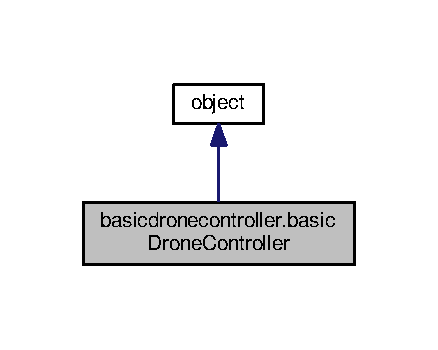
\includegraphics[width=210pt]{classbasicdronecontroller_1_1basicDroneController__inherit__graph}
\end{center}
\end{figure}


Collaboration diagram for basicdronecontroller.\-basic\-Drone\-Controller\-:
\nopagebreak
\begin{figure}[H]
\begin{center}
\leavevmode
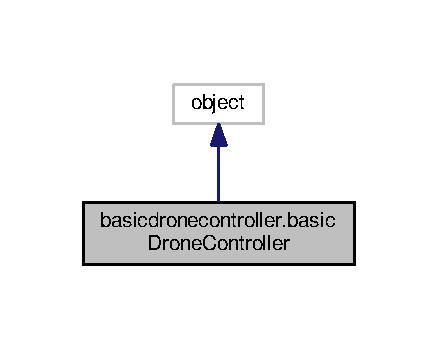
\includegraphics[width=234pt]{classbasicdronecontroller_1_1basicDroneController__coll__graph}
\end{center}
\end{figure}
\subsection*{Public Member Functions}
\begin{DoxyCompactItemize}
\item 
def \hyperlink{classbasicdronecontroller_1_1basicDroneController_a9bd81e29fd08aadc783b88741927d37a}{\-\_\-\-\_\-init\-\_\-\-\_\-}
\item 
def \hyperlink{classbasicdronecontroller_1_1basicDroneController_acd648a8a012fc871ab85d600ef5b4076}{receive\-Navdata}
\item 
def \hyperlink{classbasicdronecontroller_1_1basicDroneController_aa9322ef1dca7727b1fa406a4a590753d}{sendtakeoff}
\item 
def \hyperlink{classbasicdronecontroller_1_1basicDroneController_ae5a8f73cf76fcb94cf90b10df1252a80}{send\-Land}
\item 
def \hyperlink{classbasicdronecontroller_1_1basicDroneController_a1c23d1454ad676473271933e8d6ec2fa}{send\-Emergency}
\item 
def \hyperlink{classbasicdronecontroller_1_1basicDroneController_a34f77a0edfe08f4aa8c2d92dc7141a7e}{set\-Command}
\item 
def \hyperlink{classbasicdronecontroller_1_1basicDroneController_af7a7f58aa7fc27e4e26e53c521dd30d1}{send\-Command}
\item 
def \hyperlink{classbasicdronecontroller_1_1basicDroneController_ac1fdffd4ba5cdd00b830742d3223b402}{land\-Before\-Exit}
\end{DoxyCompactItemize}
\subsection*{Public Attributes}
\begin{DoxyCompactItemize}
\item 
\hyperlink{classbasicdronecontroller_1_1basicDroneController_a18e9a784471aeea334924200a3436ea0}{status}
\item 
\hyperlink{classbasicdronecontroller_1_1basicDroneController_adf8d9672e3056c0d4efe910a88d21aa6}{P\-A\-T\-H}
\item 
\hyperlink{classbasicdronecontroller_1_1basicDroneController_a29958b85ade2a93b5c860430147e9899}{C\-O\-M\-M\-A\-N\-D\-\_\-\-P\-E\-R\-I\-O\-D}
\item 
\hyperlink{classbasicdronecontroller_1_1basicDroneController_a182cc9c8459937f8db8ff30f666234b9}{sub\-Navdata}
\item 
\hyperlink{classbasicdronecontroller_1_1basicDroneController_aa26852e9bc4b9a8a78639a7973a0037f}{pub\-Land}
\item 
\hyperlink{classbasicdronecontroller_1_1basicDroneController_a65bf2f7ffe2d7408d865e4b3cdc6bbdf}{pubtakeoff}
\item 
\hyperlink{classbasicdronecontroller_1_1basicDroneController_ab960a8784bab6e3c99204893f2a4a910}{pub\-Reset}
\item 
\hyperlink{classbasicdronecontroller_1_1basicDroneController_ad6b79da799e584a1d6f06e472f06fab2}{pub\-Command}
\item 
\hyperlink{classbasicdronecontroller_1_1basicDroneController_a61307b396db405d7a75e9ac310abc1c9}{command}
\item 
\hyperlink{classbasicdronecontroller_1_1basicDroneController_aec39e95fe93747f72ac864717480dcb4}{command\-Timer}
\end{DoxyCompactItemize}
\subsection*{Static Public Attributes}
\begin{DoxyCompactItemize}
\item 
string \hyperlink{classbasicdronecontroller_1_1basicDroneController_ae6fe1e6547cc0b52d85acbdea802a915}{controller\-Select} = \char`\"{}None\char`\"{}
\end{DoxyCompactItemize}


\subsection{Detailed Description}


Definition at line 20 of file basicdronecontroller.\-py.



\subsection{Constructor \& Destructor Documentation}
\hypertarget{classbasicdronecontroller_1_1basicDroneController_a9bd81e29fd08aadc783b88741927d37a}{\index{basicdronecontroller\-::basic\-Drone\-Controller@{basicdronecontroller\-::basic\-Drone\-Controller}!\-\_\-\-\_\-init\-\_\-\-\_\-@{\-\_\-\-\_\-init\-\_\-\-\_\-}}
\index{\-\_\-\-\_\-init\-\_\-\-\_\-@{\-\_\-\-\_\-init\-\_\-\-\_\-}!basicdronecontroller::basicDroneController@{basicdronecontroller\-::basic\-Drone\-Controller}}
\subsubsection[{\-\_\-\-\_\-init\-\_\-\-\_\-}]{\setlength{\rightskip}{0pt plus 5cm}def basicdronecontroller.\-basic\-Drone\-Controller.\-\_\-\-\_\-init\-\_\-\-\_\- (
\begin{DoxyParamCaption}
\item[{}]{self}
\end{DoxyParamCaption}
)}}\label{classbasicdronecontroller_1_1basicDroneController_a9bd81e29fd08aadc783b88741927d37a}


Definition at line 23 of file basicdronecontroller.\-py.



\subsection{Member Function Documentation}
\hypertarget{classbasicdronecontroller_1_1basicDroneController_ac1fdffd4ba5cdd00b830742d3223b402}{\index{basicdronecontroller\-::basic\-Drone\-Controller@{basicdronecontroller\-::basic\-Drone\-Controller}!land\-Before\-Exit@{land\-Before\-Exit}}
\index{land\-Before\-Exit@{land\-Before\-Exit}!basicdronecontroller::basicDroneController@{basicdronecontroller\-::basic\-Drone\-Controller}}
\subsubsection[{land\-Before\-Exit}]{\setlength{\rightskip}{0pt plus 5cm}def basicdronecontroller.\-basic\-Drone\-Controller.\-land\-Before\-Exit (
\begin{DoxyParamCaption}
\item[{}]{self}
\end{DoxyParamCaption}
)}}\label{classbasicdronecontroller_1_1basicDroneController_ac1fdffd4ba5cdd00b830742d3223b402}


Definition at line 83 of file basicdronecontroller.\-py.

\hypertarget{classbasicdronecontroller_1_1basicDroneController_acd648a8a012fc871ab85d600ef5b4076}{\index{basicdronecontroller\-::basic\-Drone\-Controller@{basicdronecontroller\-::basic\-Drone\-Controller}!receive\-Navdata@{receive\-Navdata}}
\index{receive\-Navdata@{receive\-Navdata}!basicdronecontroller::basicDroneController@{basicdronecontroller\-::basic\-Drone\-Controller}}
\subsubsection[{receive\-Navdata}]{\setlength{\rightskip}{0pt plus 5cm}def basicdronecontroller.\-basic\-Drone\-Controller.\-receive\-Navdata (
\begin{DoxyParamCaption}
\item[{}]{self, }
\item[{}]{navdata}
\end{DoxyParamCaption}
)}}\label{classbasicdronecontroller_1_1basicDroneController_acd648a8a012fc871ab85d600ef5b4076}


Definition at line 47 of file basicdronecontroller.\-py.

\hypertarget{classbasicdronecontroller_1_1basicDroneController_af7a7f58aa7fc27e4e26e53c521dd30d1}{\index{basicdronecontroller\-::basic\-Drone\-Controller@{basicdronecontroller\-::basic\-Drone\-Controller}!send\-Command@{send\-Command}}
\index{send\-Command@{send\-Command}!basicdronecontroller::basicDroneController@{basicdronecontroller\-::basic\-Drone\-Controller}}
\subsubsection[{send\-Command}]{\setlength{\rightskip}{0pt plus 5cm}def basicdronecontroller.\-basic\-Drone\-Controller.\-send\-Command (
\begin{DoxyParamCaption}
\item[{}]{self, }
\item[{}]{event}
\end{DoxyParamCaption}
)}}\label{classbasicdronecontroller_1_1basicDroneController_af7a7f58aa7fc27e4e26e53c521dd30d1}


Definition at line 78 of file basicdronecontroller.\-py.

\hypertarget{classbasicdronecontroller_1_1basicDroneController_a1c23d1454ad676473271933e8d6ec2fa}{\index{basicdronecontroller\-::basic\-Drone\-Controller@{basicdronecontroller\-::basic\-Drone\-Controller}!send\-Emergency@{send\-Emergency}}
\index{send\-Emergency@{send\-Emergency}!basicdronecontroller::basicDroneController@{basicdronecontroller\-::basic\-Drone\-Controller}}
\subsubsection[{send\-Emergency}]{\setlength{\rightskip}{0pt plus 5cm}def basicdronecontroller.\-basic\-Drone\-Controller.\-send\-Emergency (
\begin{DoxyParamCaption}
\item[{}]{self, }
\item[{}]{I\-D}
\end{DoxyParamCaption}
)}}\label{classbasicdronecontroller_1_1basicDroneController_a1c23d1454ad676473271933e8d6ec2fa}


Definition at line 63 of file basicdronecontroller.\-py.

\hypertarget{classbasicdronecontroller_1_1basicDroneController_ae5a8f73cf76fcb94cf90b10df1252a80}{\index{basicdronecontroller\-::basic\-Drone\-Controller@{basicdronecontroller\-::basic\-Drone\-Controller}!send\-Land@{send\-Land}}
\index{send\-Land@{send\-Land}!basicdronecontroller::basicDroneController@{basicdronecontroller\-::basic\-Drone\-Controller}}
\subsubsection[{send\-Land}]{\setlength{\rightskip}{0pt plus 5cm}def basicdronecontroller.\-basic\-Drone\-Controller.\-send\-Land (
\begin{DoxyParamCaption}
\item[{}]{self, }
\item[{}]{I\-D}
\end{DoxyParamCaption}
)}}\label{classbasicdronecontroller_1_1basicDroneController_ae5a8f73cf76fcb94cf90b10df1252a80}


Definition at line 57 of file basicdronecontroller.\-py.

\hypertarget{classbasicdronecontroller_1_1basicDroneController_aa9322ef1dca7727b1fa406a4a590753d}{\index{basicdronecontroller\-::basic\-Drone\-Controller@{basicdronecontroller\-::basic\-Drone\-Controller}!sendtakeoff@{sendtakeoff}}
\index{sendtakeoff@{sendtakeoff}!basicdronecontroller::basicDroneController@{basicdronecontroller\-::basic\-Drone\-Controller}}
\subsubsection[{sendtakeoff}]{\setlength{\rightskip}{0pt plus 5cm}def basicdronecontroller.\-basic\-Drone\-Controller.\-sendtakeoff (
\begin{DoxyParamCaption}
\item[{}]{self, }
\item[{}]{I\-D}
\end{DoxyParamCaption}
)}}\label{classbasicdronecontroller_1_1basicDroneController_aa9322ef1dca7727b1fa406a4a590753d}


Definition at line 51 of file basicdronecontroller.\-py.

\hypertarget{classbasicdronecontroller_1_1basicDroneController_a34f77a0edfe08f4aa8c2d92dc7141a7e}{\index{basicdronecontroller\-::basic\-Drone\-Controller@{basicdronecontroller\-::basic\-Drone\-Controller}!set\-Command@{set\-Command}}
\index{set\-Command@{set\-Command}!basicdronecontroller::basicDroneController@{basicdronecontroller\-::basic\-Drone\-Controller}}
\subsubsection[{set\-Command}]{\setlength{\rightskip}{0pt plus 5cm}def basicdronecontroller.\-basic\-Drone\-Controller.\-set\-Command (
\begin{DoxyParamCaption}
\item[{}]{self, }
\item[{}]{roll = {\ttfamily 0}, }
\item[{}]{pitch = {\ttfamily 0}, }
\item[{}]{yaw\-\_\-velocity = {\ttfamily 0}, }
\item[{}]{z\-\_\-velocity = {\ttfamily 0}, }
\item[{}]{I\-D = {\ttfamily \char`\"{}None\char`\"{}}}
\end{DoxyParamCaption}
)}}\label{classbasicdronecontroller_1_1basicDroneController_a34f77a0edfe08f4aa8c2d92dc7141a7e}


Definition at line 68 of file basicdronecontroller.\-py.



\subsection{Member Data Documentation}
\hypertarget{classbasicdronecontroller_1_1basicDroneController_a61307b396db405d7a75e9ac310abc1c9}{\index{basicdronecontroller\-::basic\-Drone\-Controller@{basicdronecontroller\-::basic\-Drone\-Controller}!command@{command}}
\index{command@{command}!basicdronecontroller::basicDroneController@{basicdronecontroller\-::basic\-Drone\-Controller}}
\subsubsection[{command}]{\setlength{\rightskip}{0pt plus 5cm}basicdronecontroller.\-basic\-Drone\-Controller.\-command}}\label{classbasicdronecontroller_1_1basicDroneController_a61307b396db405d7a75e9ac310abc1c9}


Definition at line 41 of file basicdronecontroller.\-py.

\hypertarget{classbasicdronecontroller_1_1basicDroneController_a29958b85ade2a93b5c860430147e9899}{\index{basicdronecontroller\-::basic\-Drone\-Controller@{basicdronecontroller\-::basic\-Drone\-Controller}!C\-O\-M\-M\-A\-N\-D\-\_\-\-P\-E\-R\-I\-O\-D@{C\-O\-M\-M\-A\-N\-D\-\_\-\-P\-E\-R\-I\-O\-D}}
\index{C\-O\-M\-M\-A\-N\-D\-\_\-\-P\-E\-R\-I\-O\-D@{C\-O\-M\-M\-A\-N\-D\-\_\-\-P\-E\-R\-I\-O\-D}!basicdronecontroller::basicDroneController@{basicdronecontroller\-::basic\-Drone\-Controller}}
\subsubsection[{C\-O\-M\-M\-A\-N\-D\-\_\-\-P\-E\-R\-I\-O\-D}]{\setlength{\rightskip}{0pt plus 5cm}basicdronecontroller.\-basic\-Drone\-Controller.\-C\-O\-M\-M\-A\-N\-D\-\_\-\-P\-E\-R\-I\-O\-D}}\label{classbasicdronecontroller_1_1basicDroneController_a29958b85ade2a93b5c860430147e9899}


Definition at line 28 of file basicdronecontroller.\-py.

\hypertarget{classbasicdronecontroller_1_1basicDroneController_aec39e95fe93747f72ac864717480dcb4}{\index{basicdronecontroller\-::basic\-Drone\-Controller@{basicdronecontroller\-::basic\-Drone\-Controller}!command\-Timer@{command\-Timer}}
\index{command\-Timer@{command\-Timer}!basicdronecontroller::basicDroneController@{basicdronecontroller\-::basic\-Drone\-Controller}}
\subsubsection[{command\-Timer}]{\setlength{\rightskip}{0pt plus 5cm}basicdronecontroller.\-basic\-Drone\-Controller.\-command\-Timer}}\label{classbasicdronecontroller_1_1basicDroneController_aec39e95fe93747f72ac864717480dcb4}


Definition at line 42 of file basicdronecontroller.\-py.

\hypertarget{classbasicdronecontroller_1_1basicDroneController_ae6fe1e6547cc0b52d85acbdea802a915}{\index{basicdronecontroller\-::basic\-Drone\-Controller@{basicdronecontroller\-::basic\-Drone\-Controller}!controller\-Select@{controller\-Select}}
\index{controller\-Select@{controller\-Select}!basicdronecontroller::basicDroneController@{basicdronecontroller\-::basic\-Drone\-Controller}}
\subsubsection[{controller\-Select}]{\setlength{\rightskip}{0pt plus 5cm}string basicdronecontroller.\-basic\-Drone\-Controller.\-controller\-Select = \char`\"{}None\char`\"{}\hspace{0.3cm}{\ttfamily [static]}}}\label{classbasicdronecontroller_1_1basicDroneController_ae6fe1e6547cc0b52d85acbdea802a915}


Definition at line 21 of file basicdronecontroller.\-py.

\hypertarget{classbasicdronecontroller_1_1basicDroneController_adf8d9672e3056c0d4efe910a88d21aa6}{\index{basicdronecontroller\-::basic\-Drone\-Controller@{basicdronecontroller\-::basic\-Drone\-Controller}!P\-A\-T\-H@{P\-A\-T\-H}}
\index{P\-A\-T\-H@{P\-A\-T\-H}!basicdronecontroller::basicDroneController@{basicdronecontroller\-::basic\-Drone\-Controller}}
\subsubsection[{P\-A\-T\-H}]{\setlength{\rightskip}{0pt plus 5cm}basicdronecontroller.\-basic\-Drone\-Controller.\-P\-A\-T\-H}}\label{classbasicdronecontroller_1_1basicDroneController_adf8d9672e3056c0d4efe910a88d21aa6}


Definition at line 27 of file basicdronecontroller.\-py.

\hypertarget{classbasicdronecontroller_1_1basicDroneController_ad6b79da799e584a1d6f06e472f06fab2}{\index{basicdronecontroller\-::basic\-Drone\-Controller@{basicdronecontroller\-::basic\-Drone\-Controller}!pub\-Command@{pub\-Command}}
\index{pub\-Command@{pub\-Command}!basicdronecontroller::basicDroneController@{basicdronecontroller\-::basic\-Drone\-Controller}}
\subsubsection[{pub\-Command}]{\setlength{\rightskip}{0pt plus 5cm}basicdronecontroller.\-basic\-Drone\-Controller.\-pub\-Command}}\label{classbasicdronecontroller_1_1basicDroneController_ad6b79da799e584a1d6f06e472f06fab2}


Definition at line 38 of file basicdronecontroller.\-py.

\hypertarget{classbasicdronecontroller_1_1basicDroneController_aa26852e9bc4b9a8a78639a7973a0037f}{\index{basicdronecontroller\-::basic\-Drone\-Controller@{basicdronecontroller\-::basic\-Drone\-Controller}!pub\-Land@{pub\-Land}}
\index{pub\-Land@{pub\-Land}!basicdronecontroller::basicDroneController@{basicdronecontroller\-::basic\-Drone\-Controller}}
\subsubsection[{pub\-Land}]{\setlength{\rightskip}{0pt plus 5cm}basicdronecontroller.\-basic\-Drone\-Controller.\-pub\-Land}}\label{classbasicdronecontroller_1_1basicDroneController_aa26852e9bc4b9a8a78639a7973a0037f}


Definition at line 33 of file basicdronecontroller.\-py.

\hypertarget{classbasicdronecontroller_1_1basicDroneController_ab960a8784bab6e3c99204893f2a4a910}{\index{basicdronecontroller\-::basic\-Drone\-Controller@{basicdronecontroller\-::basic\-Drone\-Controller}!pub\-Reset@{pub\-Reset}}
\index{pub\-Reset@{pub\-Reset}!basicdronecontroller::basicDroneController@{basicdronecontroller\-::basic\-Drone\-Controller}}
\subsubsection[{pub\-Reset}]{\setlength{\rightskip}{0pt plus 5cm}basicdronecontroller.\-basic\-Drone\-Controller.\-pub\-Reset}}\label{classbasicdronecontroller_1_1basicDroneController_ab960a8784bab6e3c99204893f2a4a910}


Definition at line 35 of file basicdronecontroller.\-py.

\hypertarget{classbasicdronecontroller_1_1basicDroneController_a65bf2f7ffe2d7408d865e4b3cdc6bbdf}{\index{basicdronecontroller\-::basic\-Drone\-Controller@{basicdronecontroller\-::basic\-Drone\-Controller}!pubtakeoff@{pubtakeoff}}
\index{pubtakeoff@{pubtakeoff}!basicdronecontroller::basicDroneController@{basicdronecontroller\-::basic\-Drone\-Controller}}
\subsubsection[{pubtakeoff}]{\setlength{\rightskip}{0pt plus 5cm}basicdronecontroller.\-basic\-Drone\-Controller.\-pubtakeoff}}\label{classbasicdronecontroller_1_1basicDroneController_a65bf2f7ffe2d7408d865e4b3cdc6bbdf}


Definition at line 34 of file basicdronecontroller.\-py.

\hypertarget{classbasicdronecontroller_1_1basicDroneController_a18e9a784471aeea334924200a3436ea0}{\index{basicdronecontroller\-::basic\-Drone\-Controller@{basicdronecontroller\-::basic\-Drone\-Controller}!status@{status}}
\index{status@{status}!basicdronecontroller::basicDroneController@{basicdronecontroller\-::basic\-Drone\-Controller}}
\subsubsection[{status}]{\setlength{\rightskip}{0pt plus 5cm}basicdronecontroller.\-basic\-Drone\-Controller.\-status}}\label{classbasicdronecontroller_1_1basicDroneController_a18e9a784471aeea334924200a3436ea0}


Definition at line 25 of file basicdronecontroller.\-py.

\hypertarget{classbasicdronecontroller_1_1basicDroneController_a182cc9c8459937f8db8ff30f666234b9}{\index{basicdronecontroller\-::basic\-Drone\-Controller@{basicdronecontroller\-::basic\-Drone\-Controller}!sub\-Navdata@{sub\-Navdata}}
\index{sub\-Navdata@{sub\-Navdata}!basicdronecontroller::basicDroneController@{basicdronecontroller\-::basic\-Drone\-Controller}}
\subsubsection[{sub\-Navdata}]{\setlength{\rightskip}{0pt plus 5cm}basicdronecontroller.\-basic\-Drone\-Controller.\-sub\-Navdata}}\label{classbasicdronecontroller_1_1basicDroneController_a182cc9c8459937f8db8ff30f666234b9}


Definition at line 30 of file basicdronecontroller.\-py.



The documentation for this class was generated from the following file\-:\begin{DoxyCompactItemize}
\item 
\hyperlink{basicdronecontroller_8py}{basicdronecontroller.\-py}\end{DoxyCompactItemize}

\hypertarget{classclusterClass_1_1Cluster}{\section{cluster\-Class.\-Cluster Class Reference}
\label{classclusterClass_1_1Cluster}\index{cluster\-Class.\-Cluster@{cluster\-Class.\-Cluster}}
}


The documentation for this class was generated from the following file\-:\begin{DoxyCompactItemize}
\item 
cluster\-Class.\-py\end{DoxyCompactItemize}

\hypertarget{classclusterClass_1_1clusterNode}{\section{cluster\-Class.\-cluster\-Node Class Reference}
\label{classclusterClass_1_1clusterNode}\index{cluster\-Class.\-cluster\-Node@{cluster\-Class.\-cluster\-Node}}
}
\subsection*{Public Member Functions}
\begin{DoxyCompactItemize}
\item 
def \hyperlink{classclusterClass_1_1clusterNode_a0a55dbea69dafd2ce390e30c1f29c2c5}{\-\_\-\-\_\-init\-\_\-\-\_\-}
\item 
def \hyperlink{classclusterClass_1_1clusterNode_a4c4a2f70ae0a9567bd355f98774dbf92}{process\-Points}
\end{DoxyCompactItemize}


\subsection{Constructor \& Destructor Documentation}
\hypertarget{classclusterClass_1_1clusterNode_a0a55dbea69dafd2ce390e30c1f29c2c5}{\index{cluster\-Class\-::cluster\-Node@{cluster\-Class\-::cluster\-Node}!\-\_\-\-\_\-init\-\_\-\-\_\-@{\-\_\-\-\_\-init\-\_\-\-\_\-}}
\index{\-\_\-\-\_\-init\-\_\-\-\_\-@{\-\_\-\-\_\-init\-\_\-\-\_\-}!clusterClass::clusterNode@{cluster\-Class\-::cluster\-Node}}
\subsubsection[{\-\_\-\-\_\-init\-\_\-\-\_\-}]{\setlength{\rightskip}{0pt plus 5cm}def cluster\-Class.\-cluster\-Node.\-\_\-\-\_\-init\-\_\-\-\_\- (
\begin{DoxyParamCaption}
\item[{}]{self, }
\item[{}]{linkage, }
\item[{}]{agglo\-\_\-cutoff}
\end{DoxyParamCaption}
)}}\label{classclusterClass_1_1clusterNode_a0a55dbea69dafd2ce390e30c1f29c2c5}
\begin{DoxyVerb}Initialize point clustering class\end{DoxyVerb}
 

\subsection{Member Function Documentation}
\hypertarget{classclusterClass_1_1clusterNode_a4c4a2f70ae0a9567bd355f98774dbf92}{\index{cluster\-Class\-::cluster\-Node@{cluster\-Class\-::cluster\-Node}!process\-Points@{process\-Points}}
\index{process\-Points@{process\-Points}!clusterClass::clusterNode@{cluster\-Class\-::cluster\-Node}}
\subsubsection[{process\-Points}]{\setlength{\rightskip}{0pt plus 5cm}def cluster\-Class.\-cluster\-Node.\-process\-Points (
\begin{DoxyParamCaption}
\item[{}]{self, }
\item[{}]{point\-Stamped}
\end{DoxyParamCaption}
)}}\label{classclusterClass_1_1clusterNode_a4c4a2f70ae0a9567bd355f98774dbf92}
\begin{DoxyVerb}Process incoming points. Project to '/map' coordinates and puts them into an array\end{DoxyVerb}
 

The documentation for this class was generated from the following file\-:\begin{DoxyCompactItemize}
\item 
cluster\-Class.\-py\end{DoxyCompactItemize}

\hypertarget{classbasicdronecontroller_1_1droneStatus}{\section{basicdronecontroller.\-drone\-Status Class Reference}
\label{classbasicdronecontroller_1_1droneStatus}\index{basicdronecontroller.\-drone\-Status@{basicdronecontroller.\-drone\-Status}}
}


Inheritance diagram for basicdronecontroller.\-drone\-Status\-:
\nopagebreak
\begin{figure}[H]
\begin{center}
\leavevmode
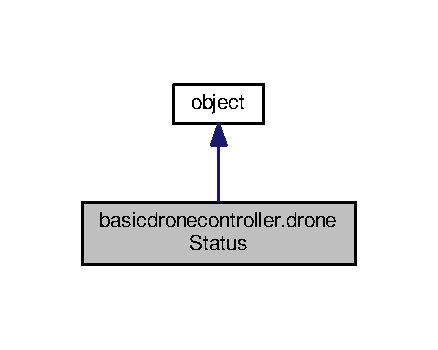
\includegraphics[width=210pt]{classbasicdronecontroller_1_1droneStatus__inherit__graph}
\end{center}
\end{figure}


Collaboration diagram for basicdronecontroller.\-drone\-Status\-:
\nopagebreak
\begin{figure}[H]
\begin{center}
\leavevmode
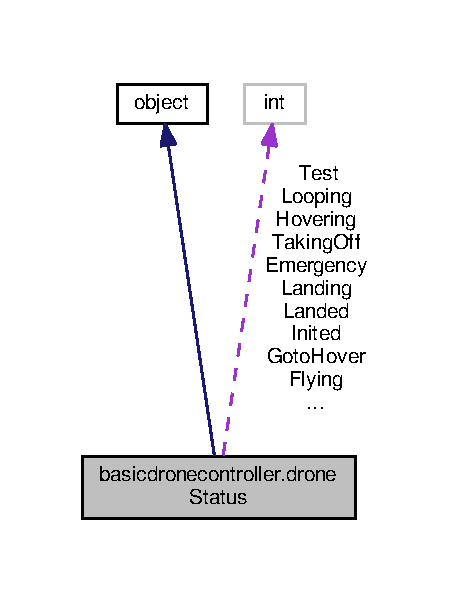
\includegraphics[width=217pt]{classbasicdronecontroller_1_1droneStatus__coll__graph}
\end{center}
\end{figure}
\subsection*{Static Public Attributes}
\begin{DoxyCompactItemize}
\item 
int \hyperlink{classbasicdronecontroller_1_1droneStatus_aac1e2fb427e0e18858ce2066819ad0b2}{Emergency} = 0
\item 
int \hyperlink{classbasicdronecontroller_1_1droneStatus_a863d58782e3420a6d75708af2918cd62}{Inited} = 1
\item 
int \hyperlink{classbasicdronecontroller_1_1droneStatus_a000dd254bab4b0e9b269b3890e3332c3}{Landed} = 2
\item 
int \hyperlink{classbasicdronecontroller_1_1droneStatus_a5d0bf13223a3b7a124ffaffbdb3dc64b}{Flying} = 3
\item 
int \hyperlink{classbasicdronecontroller_1_1droneStatus_ae3e6d81aa58b0c268e4084606686317d}{Hovering} = 4
\item 
int \hyperlink{classbasicdronecontroller_1_1droneStatus_a9d9bfd54b7f837f4855e4cacb9cfb089}{Test} = 5
\item 
int \hyperlink{classbasicdronecontroller_1_1droneStatus_a922dc19950f805d567027f609b880e29}{Taking\-Off} = 6
\item 
int \hyperlink{classbasicdronecontroller_1_1droneStatus_a9ad6b5e9db4ee151a3547a9e89c5289e}{Goto\-Hover} = 7
\item 
int \hyperlink{classbasicdronecontroller_1_1droneStatus_a81c1b21b3a885042dc0eabf2dfb8366e}{Landing} = 8
\item 
int \hyperlink{classbasicdronecontroller_1_1droneStatus_a17f3b8ae27dc6906ca523270a2247975}{Looping} = 9
\end{DoxyCompactItemize}


\subsection{Detailed Description}


Definition at line 8 of file basicdronecontroller.\-py.



\subsection{Member Data Documentation}
\hypertarget{classbasicdronecontroller_1_1droneStatus_aac1e2fb427e0e18858ce2066819ad0b2}{\index{basicdronecontroller\-::drone\-Status@{basicdronecontroller\-::drone\-Status}!Emergency@{Emergency}}
\index{Emergency@{Emergency}!basicdronecontroller::droneStatus@{basicdronecontroller\-::drone\-Status}}
\subsubsection[{Emergency}]{\setlength{\rightskip}{0pt plus 5cm}int basicdronecontroller.\-drone\-Status.\-Emergency = 0\hspace{0.3cm}{\ttfamily [static]}}}\label{classbasicdronecontroller_1_1droneStatus_aac1e2fb427e0e18858ce2066819ad0b2}


Definition at line 9 of file basicdronecontroller.\-py.

\hypertarget{classbasicdronecontroller_1_1droneStatus_a5d0bf13223a3b7a124ffaffbdb3dc64b}{\index{basicdronecontroller\-::drone\-Status@{basicdronecontroller\-::drone\-Status}!Flying@{Flying}}
\index{Flying@{Flying}!basicdronecontroller::droneStatus@{basicdronecontroller\-::drone\-Status}}
\subsubsection[{Flying}]{\setlength{\rightskip}{0pt plus 5cm}int basicdronecontroller.\-drone\-Status.\-Flying = 3\hspace{0.3cm}{\ttfamily [static]}}}\label{classbasicdronecontroller_1_1droneStatus_a5d0bf13223a3b7a124ffaffbdb3dc64b}


Definition at line 12 of file basicdronecontroller.\-py.

\hypertarget{classbasicdronecontroller_1_1droneStatus_a9ad6b5e9db4ee151a3547a9e89c5289e}{\index{basicdronecontroller\-::drone\-Status@{basicdronecontroller\-::drone\-Status}!Goto\-Hover@{Goto\-Hover}}
\index{Goto\-Hover@{Goto\-Hover}!basicdronecontroller::droneStatus@{basicdronecontroller\-::drone\-Status}}
\subsubsection[{Goto\-Hover}]{\setlength{\rightskip}{0pt plus 5cm}int basicdronecontroller.\-drone\-Status.\-Goto\-Hover = 7\hspace{0.3cm}{\ttfamily [static]}}}\label{classbasicdronecontroller_1_1droneStatus_a9ad6b5e9db4ee151a3547a9e89c5289e}


Definition at line 16 of file basicdronecontroller.\-py.

\hypertarget{classbasicdronecontroller_1_1droneStatus_ae3e6d81aa58b0c268e4084606686317d}{\index{basicdronecontroller\-::drone\-Status@{basicdronecontroller\-::drone\-Status}!Hovering@{Hovering}}
\index{Hovering@{Hovering}!basicdronecontroller::droneStatus@{basicdronecontroller\-::drone\-Status}}
\subsubsection[{Hovering}]{\setlength{\rightskip}{0pt plus 5cm}int basicdronecontroller.\-drone\-Status.\-Hovering = 4\hspace{0.3cm}{\ttfamily [static]}}}\label{classbasicdronecontroller_1_1droneStatus_ae3e6d81aa58b0c268e4084606686317d}


Definition at line 13 of file basicdronecontroller.\-py.

\hypertarget{classbasicdronecontroller_1_1droneStatus_a863d58782e3420a6d75708af2918cd62}{\index{basicdronecontroller\-::drone\-Status@{basicdronecontroller\-::drone\-Status}!Inited@{Inited}}
\index{Inited@{Inited}!basicdronecontroller::droneStatus@{basicdronecontroller\-::drone\-Status}}
\subsubsection[{Inited}]{\setlength{\rightskip}{0pt plus 5cm}int basicdronecontroller.\-drone\-Status.\-Inited = 1\hspace{0.3cm}{\ttfamily [static]}}}\label{classbasicdronecontroller_1_1droneStatus_a863d58782e3420a6d75708af2918cd62}


Definition at line 10 of file basicdronecontroller.\-py.

\hypertarget{classbasicdronecontroller_1_1droneStatus_a000dd254bab4b0e9b269b3890e3332c3}{\index{basicdronecontroller\-::drone\-Status@{basicdronecontroller\-::drone\-Status}!Landed@{Landed}}
\index{Landed@{Landed}!basicdronecontroller::droneStatus@{basicdronecontroller\-::drone\-Status}}
\subsubsection[{Landed}]{\setlength{\rightskip}{0pt plus 5cm}int basicdronecontroller.\-drone\-Status.\-Landed = 2\hspace{0.3cm}{\ttfamily [static]}}}\label{classbasicdronecontroller_1_1droneStatus_a000dd254bab4b0e9b269b3890e3332c3}


Definition at line 11 of file basicdronecontroller.\-py.

\hypertarget{classbasicdronecontroller_1_1droneStatus_a81c1b21b3a885042dc0eabf2dfb8366e}{\index{basicdronecontroller\-::drone\-Status@{basicdronecontroller\-::drone\-Status}!Landing@{Landing}}
\index{Landing@{Landing}!basicdronecontroller::droneStatus@{basicdronecontroller\-::drone\-Status}}
\subsubsection[{Landing}]{\setlength{\rightskip}{0pt plus 5cm}int basicdronecontroller.\-drone\-Status.\-Landing = 8\hspace{0.3cm}{\ttfamily [static]}}}\label{classbasicdronecontroller_1_1droneStatus_a81c1b21b3a885042dc0eabf2dfb8366e}


Definition at line 17 of file basicdronecontroller.\-py.

\hypertarget{classbasicdronecontroller_1_1droneStatus_a17f3b8ae27dc6906ca523270a2247975}{\index{basicdronecontroller\-::drone\-Status@{basicdronecontroller\-::drone\-Status}!Looping@{Looping}}
\index{Looping@{Looping}!basicdronecontroller::droneStatus@{basicdronecontroller\-::drone\-Status}}
\subsubsection[{Looping}]{\setlength{\rightskip}{0pt plus 5cm}int basicdronecontroller.\-drone\-Status.\-Looping = 9\hspace{0.3cm}{\ttfamily [static]}}}\label{classbasicdronecontroller_1_1droneStatus_a17f3b8ae27dc6906ca523270a2247975}


Definition at line 18 of file basicdronecontroller.\-py.

\hypertarget{classbasicdronecontroller_1_1droneStatus_a922dc19950f805d567027f609b880e29}{\index{basicdronecontroller\-::drone\-Status@{basicdronecontroller\-::drone\-Status}!Taking\-Off@{Taking\-Off}}
\index{Taking\-Off@{Taking\-Off}!basicdronecontroller::droneStatus@{basicdronecontroller\-::drone\-Status}}
\subsubsection[{Taking\-Off}]{\setlength{\rightskip}{0pt plus 5cm}int basicdronecontroller.\-drone\-Status.\-Taking\-Off = 6\hspace{0.3cm}{\ttfamily [static]}}}\label{classbasicdronecontroller_1_1droneStatus_a922dc19950f805d567027f609b880e29}


Definition at line 15 of file basicdronecontroller.\-py.

\hypertarget{classbasicdronecontroller_1_1droneStatus_a9d9bfd54b7f837f4855e4cacb9cfb089}{\index{basicdronecontroller\-::drone\-Status@{basicdronecontroller\-::drone\-Status}!Test@{Test}}
\index{Test@{Test}!basicdronecontroller::droneStatus@{basicdronecontroller\-::drone\-Status}}
\subsubsection[{Test}]{\setlength{\rightskip}{0pt plus 5cm}int basicdronecontroller.\-drone\-Status.\-Test = 5\hspace{0.3cm}{\ttfamily [static]}}}\label{classbasicdronecontroller_1_1droneStatus_a9d9bfd54b7f837f4855e4cacb9cfb089}


Definition at line 14 of file basicdronecontroller.\-py.



The documentation for this class was generated from the following file\-:\begin{DoxyCompactItemize}
\item 
\hyperlink{basicdronecontroller_8py}{basicdronecontroller.\-py}\end{DoxyCompactItemize}

\hypertarget{classgamepadcontroller_1_1gamepadController}{\section{gamepadcontroller.\-gamepad\-Controller Class Reference}
\label{classgamepadcontroller_1_1gamepadController}\index{gamepadcontroller.\-gamepad\-Controller@{gamepadcontroller.\-gamepad\-Controller}}
}


Collaboration diagram for gamepadcontroller.\-gamepad\-Controller\-:
\nopagebreak
\begin{figure}[H]
\begin{center}
\leavevmode
\includegraphics[width=299pt]{classgamepadcontroller_1_1gamepadController__coll__graph}
\end{center}
\end{figure}
\subsection*{Public Member Functions}
\begin{DoxyCompactItemize}
\item 
def \hyperlink{classgamepadcontroller_1_1gamepadController_a56dc7ac32e35bec7226c6555d168bf4b}{\-\_\-\-\_\-init\-\_\-\-\_\-}
\item 
def \hyperlink{classgamepadcontroller_1_1gamepadController_a18d44e0d49a0d7e4a515092b016464ef}{Receive\-Joystick\-Message}
\item 
def \hyperlink{classgamepadcontroller_1_1gamepadController_a9bd3d20beace00cd8381d708097bbf61}{close}
\end{DoxyCompactItemize}
\subsection*{Public Attributes}
\begin{DoxyCompactItemize}
\item 
\hyperlink{classgamepadcontroller_1_1gamepadController_a3f5663a47a7792c7efeee56d86eaf641}{I\-D}
\item 
\hyperlink{classgamepadcontroller_1_1gamepadController_ab004a378de876574e55c879d5ea862ec}{window}
\item 
\hyperlink{classgamepadcontroller_1_1gamepadController_a10b7595ea5c2655a9ed3ddba6f62424d}{controller}
\item 
\hyperlink{classgamepadcontroller_1_1gamepadController_aec42e233c0618abef806d0b548dec8d4}{process}
\item 
\hyperlink{classgamepadcontroller_1_1gamepadController_a59a38e68ed8c9b0e1c5e2a84987dd1db}{button\-Emergency}
\item 
\hyperlink{classgamepadcontroller_1_1gamepadController_a56184378a52735c52b4a3040e3e72f09}{button\-Land}
\item 
\hyperlink{classgamepadcontroller_1_1gamepadController_a9b7c53bfe95d03188a100b3119a1d431}{button\-Takeoff}
\item 
\hyperlink{classgamepadcontroller_1_1gamepadController_a156019a4d829536a5ebf430e8eae6204}{axis\-Roll}
\item 
\hyperlink{classgamepadcontroller_1_1gamepadController_a800de9de7b4d166b545c5dbbd411b423}{axis\-Pitch}
\item 
\hyperlink{classgamepadcontroller_1_1gamepadController_a1bf5e24ecbf94d3a4ea99dd267b548bc}{axis\-Yaw}
\item 
\hyperlink{classgamepadcontroller_1_1gamepadController_af158dff2b0b9efc973c94c50c60ac938}{axis\-Z}
\item 
\hyperlink{classgamepadcontroller_1_1gamepadController_aba4b8e93dc52cb30c7069a366ab03bcc}{scale\-Roll}
\item 
\hyperlink{classgamepadcontroller_1_1gamepadController_a02885140d6d2efc1f469e063018a8c46}{scale\-Pitch}
\item 
\hyperlink{classgamepadcontroller_1_1gamepadController_ad9e4b5c372ecf121fd1a45baba34cfb8}{scale\-Yaw}
\item 
\hyperlink{classgamepadcontroller_1_1gamepadController_a80be0bf69c042473e69428bb39988494}{scale\-Z}
\item 
\hyperlink{classgamepadcontroller_1_1gamepadController_aa6797c1d03e7d3c9aa483ae386b25c52}{sub\-Joystick}
\end{DoxyCompactItemize}
\subsection*{Static Public Attributes}
\begin{DoxyCompactItemize}
\item 
tuple \hyperlink{classgamepadcontroller_1_1gamepadController_a2058f8060f1d8406118bcf0bb5e18729}{device} = commands.\-getoutput('ls /dev/input/js$\ast$')
\item 
int \hyperlink{classgamepadcontroller_1_1gamepadController_af4f9816a1459785ead61211c503b99b8}{button\-Emergency} = 0
\item 
int \hyperlink{classgamepadcontroller_1_1gamepadController_aa6a3832d0061812df791a90a098667a9}{button\-Land} = 1
\item 
int \hyperlink{classgamepadcontroller_1_1gamepadController_a2db2148491b5738f9b7e3eff5eafce2a}{button\-Takeoff} = 2
\item 
int \hyperlink{classgamepadcontroller_1_1gamepadController_ac74e4b60b29519689493aa031d5730aa}{axis\-Roll} = 0
\item 
int \hyperlink{classgamepadcontroller_1_1gamepadController_adc709abe90153ab637e44c009df3cb00}{axis\-Pitch} = 1
\item 
int \hyperlink{classgamepadcontroller_1_1gamepadController_ab7cb1425723b9954e1857744425aebac}{axis\-Yaw} = 3
\item 
int \hyperlink{classgamepadcontroller_1_1gamepadController_acd1ac84f9fc64a8e3ad69b5904b360c9}{axis\-Z} = 4
\item 
float \hyperlink{classgamepadcontroller_1_1gamepadController_a15894d1acf2099bde66ec5869cf36724}{scale\-Roll} = 1.\-0
\item 
float \hyperlink{classgamepadcontroller_1_1gamepadController_a166739b1f1faef71ea463c544db75adf}{scale\-Pitch} = 1.\-0
\item 
float \hyperlink{classgamepadcontroller_1_1gamepadController_a5b8de0ec2f3c6f1a81997266e1b91d24}{scale\-Yaw} = 1.\-0
\item 
float \hyperlink{classgamepadcontroller_1_1gamepadController_a3d34de8357dd41a4a63cdb3dd38569d1}{scale\-Z} = 1.\-0
\end{DoxyCompactItemize}


\subsection{Detailed Description}


Definition at line 5 of file gamepadcontroller.\-py.



\subsection{Constructor \& Destructor Documentation}
\hypertarget{classgamepadcontroller_1_1gamepadController_a56dc7ac32e35bec7226c6555d168bf4b}{\index{gamepadcontroller\-::gamepad\-Controller@{gamepadcontroller\-::gamepad\-Controller}!\-\_\-\-\_\-init\-\_\-\-\_\-@{\-\_\-\-\_\-init\-\_\-\-\_\-}}
\index{\-\_\-\-\_\-init\-\_\-\-\_\-@{\-\_\-\-\_\-init\-\_\-\-\_\-}!gamepadcontroller::gamepadController@{gamepadcontroller\-::gamepad\-Controller}}
\subsubsection[{\-\_\-\-\_\-init\-\_\-\-\_\-}]{\setlength{\rightskip}{0pt plus 5cm}def gamepadcontroller.\-gamepad\-Controller.\-\_\-\-\_\-init\-\_\-\-\_\- (
\begin{DoxyParamCaption}
\item[{}]{self, }
\item[{}]{master, }
\item[{}]{C\-O\-N\-T\-R\-O\-L\-L\-E\-R}
\end{DoxyParamCaption}
)}}\label{classgamepadcontroller_1_1gamepadController_a56dc7ac32e35bec7226c6555d168bf4b}


Definition at line 27 of file gamepadcontroller.\-py.



\subsection{Member Function Documentation}
\hypertarget{classgamepadcontroller_1_1gamepadController_a9bd3d20beace00cd8381d708097bbf61}{\index{gamepadcontroller\-::gamepad\-Controller@{gamepadcontroller\-::gamepad\-Controller}!close@{close}}
\index{close@{close}!gamepadcontroller::gamepadController@{gamepadcontroller\-::gamepad\-Controller}}
\subsubsection[{close}]{\setlength{\rightskip}{0pt plus 5cm}def gamepadcontroller.\-gamepad\-Controller.\-close (
\begin{DoxyParamCaption}
\item[{}]{self}
\end{DoxyParamCaption}
)}}\label{classgamepadcontroller_1_1gamepadController_a9bd3d20beace00cd8381d708097bbf61}


Definition at line 84 of file gamepadcontroller.\-py.

\hypertarget{classgamepadcontroller_1_1gamepadController_a18d44e0d49a0d7e4a515092b016464ef}{\index{gamepadcontroller\-::gamepad\-Controller@{gamepadcontroller\-::gamepad\-Controller}!Receive\-Joystick\-Message@{Receive\-Joystick\-Message}}
\index{Receive\-Joystick\-Message@{Receive\-Joystick\-Message}!gamepadcontroller::gamepadController@{gamepadcontroller\-::gamepad\-Controller}}
\subsubsection[{Receive\-Joystick\-Message}]{\setlength{\rightskip}{0pt plus 5cm}def gamepadcontroller.\-gamepad\-Controller.\-Receive\-Joystick\-Message (
\begin{DoxyParamCaption}
\item[{}]{self, }
\item[{}]{data}
\end{DoxyParamCaption}
)}}\label{classgamepadcontroller_1_1gamepadController_a18d44e0d49a0d7e4a515092b016464ef}


Definition at line 71 of file gamepadcontroller.\-py.



\subsection{Member Data Documentation}
\hypertarget{classgamepadcontroller_1_1gamepadController_adc709abe90153ab637e44c009df3cb00}{\index{gamepadcontroller\-::gamepad\-Controller@{gamepadcontroller\-::gamepad\-Controller}!axis\-Pitch@{axis\-Pitch}}
\index{axis\-Pitch@{axis\-Pitch}!gamepadcontroller::gamepadController@{gamepadcontroller\-::gamepad\-Controller}}
\subsubsection[{axis\-Pitch}]{\setlength{\rightskip}{0pt plus 5cm}int gamepadcontroller.\-gamepad\-Controller.\-axis\-Pitch = 1\hspace{0.3cm}{\ttfamily [static]}}}\label{classgamepadcontroller_1_1gamepadController_adc709abe90153ab637e44c009df3cb00}


Definition at line 16 of file gamepadcontroller.\-py.

\hypertarget{classgamepadcontroller_1_1gamepadController_a800de9de7b4d166b545c5dbbd411b423}{\index{gamepadcontroller\-::gamepad\-Controller@{gamepadcontroller\-::gamepad\-Controller}!axis\-Pitch@{axis\-Pitch}}
\index{axis\-Pitch@{axis\-Pitch}!gamepadcontroller::gamepadController@{gamepadcontroller\-::gamepad\-Controller}}
\subsubsection[{axis\-Pitch}]{\setlength{\rightskip}{0pt plus 5cm}gamepadcontroller.\-gamepad\-Controller.\-axis\-Pitch}}\label{classgamepadcontroller_1_1gamepadController_a800de9de7b4d166b545c5dbbd411b423}


Definition at line 59 of file gamepadcontroller.\-py.

\hypertarget{classgamepadcontroller_1_1gamepadController_ac74e4b60b29519689493aa031d5730aa}{\index{gamepadcontroller\-::gamepad\-Controller@{gamepadcontroller\-::gamepad\-Controller}!axis\-Roll@{axis\-Roll}}
\index{axis\-Roll@{axis\-Roll}!gamepadcontroller::gamepadController@{gamepadcontroller\-::gamepad\-Controller}}
\subsubsection[{axis\-Roll}]{\setlength{\rightskip}{0pt plus 5cm}int gamepadcontroller.\-gamepad\-Controller.\-axis\-Roll = 0\hspace{0.3cm}{\ttfamily [static]}}}\label{classgamepadcontroller_1_1gamepadController_ac74e4b60b29519689493aa031d5730aa}


Definition at line 15 of file gamepadcontroller.\-py.

\hypertarget{classgamepadcontroller_1_1gamepadController_a156019a4d829536a5ebf430e8eae6204}{\index{gamepadcontroller\-::gamepad\-Controller@{gamepadcontroller\-::gamepad\-Controller}!axis\-Roll@{axis\-Roll}}
\index{axis\-Roll@{axis\-Roll}!gamepadcontroller::gamepadController@{gamepadcontroller\-::gamepad\-Controller}}
\subsubsection[{axis\-Roll}]{\setlength{\rightskip}{0pt plus 5cm}gamepadcontroller.\-gamepad\-Controller.\-axis\-Roll}}\label{classgamepadcontroller_1_1gamepadController_a156019a4d829536a5ebf430e8eae6204}


Definition at line 58 of file gamepadcontroller.\-py.

\hypertarget{classgamepadcontroller_1_1gamepadController_ab7cb1425723b9954e1857744425aebac}{\index{gamepadcontroller\-::gamepad\-Controller@{gamepadcontroller\-::gamepad\-Controller}!axis\-Yaw@{axis\-Yaw}}
\index{axis\-Yaw@{axis\-Yaw}!gamepadcontroller::gamepadController@{gamepadcontroller\-::gamepad\-Controller}}
\subsubsection[{axis\-Yaw}]{\setlength{\rightskip}{0pt plus 5cm}int gamepadcontroller.\-gamepad\-Controller.\-axis\-Yaw = 3\hspace{0.3cm}{\ttfamily [static]}}}\label{classgamepadcontroller_1_1gamepadController_ab7cb1425723b9954e1857744425aebac}


Definition at line 17 of file gamepadcontroller.\-py.

\hypertarget{classgamepadcontroller_1_1gamepadController_a1bf5e24ecbf94d3a4ea99dd267b548bc}{\index{gamepadcontroller\-::gamepad\-Controller@{gamepadcontroller\-::gamepad\-Controller}!axis\-Yaw@{axis\-Yaw}}
\index{axis\-Yaw@{axis\-Yaw}!gamepadcontroller::gamepadController@{gamepadcontroller\-::gamepad\-Controller}}
\subsubsection[{axis\-Yaw}]{\setlength{\rightskip}{0pt plus 5cm}gamepadcontroller.\-gamepad\-Controller.\-axis\-Yaw}}\label{classgamepadcontroller_1_1gamepadController_a1bf5e24ecbf94d3a4ea99dd267b548bc}


Definition at line 60 of file gamepadcontroller.\-py.

\hypertarget{classgamepadcontroller_1_1gamepadController_acd1ac84f9fc64a8e3ad69b5904b360c9}{\index{gamepadcontroller\-::gamepad\-Controller@{gamepadcontroller\-::gamepad\-Controller}!axis\-Z@{axis\-Z}}
\index{axis\-Z@{axis\-Z}!gamepadcontroller::gamepadController@{gamepadcontroller\-::gamepad\-Controller}}
\subsubsection[{axis\-Z}]{\setlength{\rightskip}{0pt plus 5cm}int gamepadcontroller.\-gamepad\-Controller.\-axis\-Z = 4\hspace{0.3cm}{\ttfamily [static]}}}\label{classgamepadcontroller_1_1gamepadController_acd1ac84f9fc64a8e3ad69b5904b360c9}


Definition at line 18 of file gamepadcontroller.\-py.

\hypertarget{classgamepadcontroller_1_1gamepadController_af158dff2b0b9efc973c94c50c60ac938}{\index{gamepadcontroller\-::gamepad\-Controller@{gamepadcontroller\-::gamepad\-Controller}!axis\-Z@{axis\-Z}}
\index{axis\-Z@{axis\-Z}!gamepadcontroller::gamepadController@{gamepadcontroller\-::gamepad\-Controller}}
\subsubsection[{axis\-Z}]{\setlength{\rightskip}{0pt plus 5cm}gamepadcontroller.\-gamepad\-Controller.\-axis\-Z}}\label{classgamepadcontroller_1_1gamepadController_af158dff2b0b9efc973c94c50c60ac938}


Definition at line 61 of file gamepadcontroller.\-py.

\hypertarget{classgamepadcontroller_1_1gamepadController_af4f9816a1459785ead61211c503b99b8}{\index{gamepadcontroller\-::gamepad\-Controller@{gamepadcontroller\-::gamepad\-Controller}!button\-Emergency@{button\-Emergency}}
\index{button\-Emergency@{button\-Emergency}!gamepadcontroller::gamepadController@{gamepadcontroller\-::gamepad\-Controller}}
\subsubsection[{button\-Emergency}]{\setlength{\rightskip}{0pt plus 5cm}int gamepadcontroller.\-gamepad\-Controller.\-button\-Emergency = 0\hspace{0.3cm}{\ttfamily [static]}}}\label{classgamepadcontroller_1_1gamepadController_af4f9816a1459785ead61211c503b99b8}


Definition at line 10 of file gamepadcontroller.\-py.

\hypertarget{classgamepadcontroller_1_1gamepadController_a59a38e68ed8c9b0e1c5e2a84987dd1db}{\index{gamepadcontroller\-::gamepad\-Controller@{gamepadcontroller\-::gamepad\-Controller}!button\-Emergency@{button\-Emergency}}
\index{button\-Emergency@{button\-Emergency}!gamepadcontroller::gamepadController@{gamepadcontroller\-::gamepad\-Controller}}
\subsubsection[{button\-Emergency}]{\setlength{\rightskip}{0pt plus 5cm}gamepadcontroller.\-gamepad\-Controller.\-button\-Emergency}}\label{classgamepadcontroller_1_1gamepadController_a59a38e68ed8c9b0e1c5e2a84987dd1db}


Definition at line 55 of file gamepadcontroller.\-py.

\hypertarget{classgamepadcontroller_1_1gamepadController_aa6a3832d0061812df791a90a098667a9}{\index{gamepadcontroller\-::gamepad\-Controller@{gamepadcontroller\-::gamepad\-Controller}!button\-Land@{button\-Land}}
\index{button\-Land@{button\-Land}!gamepadcontroller::gamepadController@{gamepadcontroller\-::gamepad\-Controller}}
\subsubsection[{button\-Land}]{\setlength{\rightskip}{0pt plus 5cm}int gamepadcontroller.\-gamepad\-Controller.\-button\-Land = 1\hspace{0.3cm}{\ttfamily [static]}}}\label{classgamepadcontroller_1_1gamepadController_aa6a3832d0061812df791a90a098667a9}


Definition at line 11 of file gamepadcontroller.\-py.

\hypertarget{classgamepadcontroller_1_1gamepadController_a56184378a52735c52b4a3040e3e72f09}{\index{gamepadcontroller\-::gamepad\-Controller@{gamepadcontroller\-::gamepad\-Controller}!button\-Land@{button\-Land}}
\index{button\-Land@{button\-Land}!gamepadcontroller::gamepadController@{gamepadcontroller\-::gamepad\-Controller}}
\subsubsection[{button\-Land}]{\setlength{\rightskip}{0pt plus 5cm}gamepadcontroller.\-gamepad\-Controller.\-button\-Land}}\label{classgamepadcontroller_1_1gamepadController_a56184378a52735c52b4a3040e3e72f09}


Definition at line 56 of file gamepadcontroller.\-py.

\hypertarget{classgamepadcontroller_1_1gamepadController_a2db2148491b5738f9b7e3eff5eafce2a}{\index{gamepadcontroller\-::gamepad\-Controller@{gamepadcontroller\-::gamepad\-Controller}!button\-Takeoff@{button\-Takeoff}}
\index{button\-Takeoff@{button\-Takeoff}!gamepadcontroller::gamepadController@{gamepadcontroller\-::gamepad\-Controller}}
\subsubsection[{button\-Takeoff}]{\setlength{\rightskip}{0pt plus 5cm}int gamepadcontroller.\-gamepad\-Controller.\-button\-Takeoff = 2\hspace{0.3cm}{\ttfamily [static]}}}\label{classgamepadcontroller_1_1gamepadController_a2db2148491b5738f9b7e3eff5eafce2a}


Definition at line 12 of file gamepadcontroller.\-py.

\hypertarget{classgamepadcontroller_1_1gamepadController_a9b7c53bfe95d03188a100b3119a1d431}{\index{gamepadcontroller\-::gamepad\-Controller@{gamepadcontroller\-::gamepad\-Controller}!button\-Takeoff@{button\-Takeoff}}
\index{button\-Takeoff@{button\-Takeoff}!gamepadcontroller::gamepadController@{gamepadcontroller\-::gamepad\-Controller}}
\subsubsection[{button\-Takeoff}]{\setlength{\rightskip}{0pt plus 5cm}gamepadcontroller.\-gamepad\-Controller.\-button\-Takeoff}}\label{classgamepadcontroller_1_1gamepadController_a9b7c53bfe95d03188a100b3119a1d431}


Definition at line 57 of file gamepadcontroller.\-py.

\hypertarget{classgamepadcontroller_1_1gamepadController_a10b7595ea5c2655a9ed3ddba6f62424d}{\index{gamepadcontroller\-::gamepad\-Controller@{gamepadcontroller\-::gamepad\-Controller}!controller@{controller}}
\index{controller@{controller}!gamepadcontroller::gamepadController@{gamepadcontroller\-::gamepad\-Controller}}
\subsubsection[{controller}]{\setlength{\rightskip}{0pt plus 5cm}gamepadcontroller.\-gamepad\-Controller.\-controller}}\label{classgamepadcontroller_1_1gamepadController_a10b7595ea5c2655a9ed3ddba6f62424d}


Definition at line 35 of file gamepadcontroller.\-py.

\hypertarget{classgamepadcontroller_1_1gamepadController_a2058f8060f1d8406118bcf0bb5e18729}{\index{gamepadcontroller\-::gamepad\-Controller@{gamepadcontroller\-::gamepad\-Controller}!device@{device}}
\index{device@{device}!gamepadcontroller::gamepadController@{gamepadcontroller\-::gamepad\-Controller}}
\subsubsection[{device}]{\setlength{\rightskip}{0pt plus 5cm}tuple gamepadcontroller.\-gamepad\-Controller.\-device = commands.\-getoutput('ls /dev/input/js$\ast$')\hspace{0.3cm}{\ttfamily [static]}}}\label{classgamepadcontroller_1_1gamepadController_a2058f8060f1d8406118bcf0bb5e18729}


Definition at line 7 of file gamepadcontroller.\-py.

\hypertarget{classgamepadcontroller_1_1gamepadController_a3f5663a47a7792c7efeee56d86eaf641}{\index{gamepadcontroller\-::gamepad\-Controller@{gamepadcontroller\-::gamepad\-Controller}!I\-D@{I\-D}}
\index{I\-D@{I\-D}!gamepadcontroller::gamepadController@{gamepadcontroller\-::gamepad\-Controller}}
\subsubsection[{I\-D}]{\setlength{\rightskip}{0pt plus 5cm}gamepadcontroller.\-gamepad\-Controller.\-I\-D}}\label{classgamepadcontroller_1_1gamepadController_a3f5663a47a7792c7efeee56d86eaf641}


Definition at line 28 of file gamepadcontroller.\-py.

\hypertarget{classgamepadcontroller_1_1gamepadController_aec42e233c0618abef806d0b548dec8d4}{\index{gamepadcontroller\-::gamepad\-Controller@{gamepadcontroller\-::gamepad\-Controller}!process@{process}}
\index{process@{process}!gamepadcontroller::gamepadController@{gamepadcontroller\-::gamepad\-Controller}}
\subsubsection[{process}]{\setlength{\rightskip}{0pt plus 5cm}gamepadcontroller.\-gamepad\-Controller.\-process}}\label{classgamepadcontroller_1_1gamepadController_aec42e233c0618abef806d0b548dec8d4}


Definition at line 51 of file gamepadcontroller.\-py.

\hypertarget{classgamepadcontroller_1_1gamepadController_a166739b1f1faef71ea463c544db75adf}{\index{gamepadcontroller\-::gamepad\-Controller@{gamepadcontroller\-::gamepad\-Controller}!scale\-Pitch@{scale\-Pitch}}
\index{scale\-Pitch@{scale\-Pitch}!gamepadcontroller::gamepadController@{gamepadcontroller\-::gamepad\-Controller}}
\subsubsection[{scale\-Pitch}]{\setlength{\rightskip}{0pt plus 5cm}float gamepadcontroller.\-gamepad\-Controller.\-scale\-Pitch = 1.\-0\hspace{0.3cm}{\ttfamily [static]}}}\label{classgamepadcontroller_1_1gamepadController_a166739b1f1faef71ea463c544db75adf}


Definition at line 22 of file gamepadcontroller.\-py.

\hypertarget{classgamepadcontroller_1_1gamepadController_a02885140d6d2efc1f469e063018a8c46}{\index{gamepadcontroller\-::gamepad\-Controller@{gamepadcontroller\-::gamepad\-Controller}!scale\-Pitch@{scale\-Pitch}}
\index{scale\-Pitch@{scale\-Pitch}!gamepadcontroller::gamepadController@{gamepadcontroller\-::gamepad\-Controller}}
\subsubsection[{scale\-Pitch}]{\setlength{\rightskip}{0pt plus 5cm}gamepadcontroller.\-gamepad\-Controller.\-scale\-Pitch}}\label{classgamepadcontroller_1_1gamepadController_a02885140d6d2efc1f469e063018a8c46}


Definition at line 63 of file gamepadcontroller.\-py.

\hypertarget{classgamepadcontroller_1_1gamepadController_a15894d1acf2099bde66ec5869cf36724}{\index{gamepadcontroller\-::gamepad\-Controller@{gamepadcontroller\-::gamepad\-Controller}!scale\-Roll@{scale\-Roll}}
\index{scale\-Roll@{scale\-Roll}!gamepadcontroller::gamepadController@{gamepadcontroller\-::gamepad\-Controller}}
\subsubsection[{scale\-Roll}]{\setlength{\rightskip}{0pt plus 5cm}float gamepadcontroller.\-gamepad\-Controller.\-scale\-Roll = 1.\-0\hspace{0.3cm}{\ttfamily [static]}}}\label{classgamepadcontroller_1_1gamepadController_a15894d1acf2099bde66ec5869cf36724}


Definition at line 21 of file gamepadcontroller.\-py.

\hypertarget{classgamepadcontroller_1_1gamepadController_aba4b8e93dc52cb30c7069a366ab03bcc}{\index{gamepadcontroller\-::gamepad\-Controller@{gamepadcontroller\-::gamepad\-Controller}!scale\-Roll@{scale\-Roll}}
\index{scale\-Roll@{scale\-Roll}!gamepadcontroller::gamepadController@{gamepadcontroller\-::gamepad\-Controller}}
\subsubsection[{scale\-Roll}]{\setlength{\rightskip}{0pt plus 5cm}gamepadcontroller.\-gamepad\-Controller.\-scale\-Roll}}\label{classgamepadcontroller_1_1gamepadController_aba4b8e93dc52cb30c7069a366ab03bcc}


Definition at line 62 of file gamepadcontroller.\-py.

\hypertarget{classgamepadcontroller_1_1gamepadController_a5b8de0ec2f3c6f1a81997266e1b91d24}{\index{gamepadcontroller\-::gamepad\-Controller@{gamepadcontroller\-::gamepad\-Controller}!scale\-Yaw@{scale\-Yaw}}
\index{scale\-Yaw@{scale\-Yaw}!gamepadcontroller::gamepadController@{gamepadcontroller\-::gamepad\-Controller}}
\subsubsection[{scale\-Yaw}]{\setlength{\rightskip}{0pt plus 5cm}float gamepadcontroller.\-gamepad\-Controller.\-scale\-Yaw = 1.\-0\hspace{0.3cm}{\ttfamily [static]}}}\label{classgamepadcontroller_1_1gamepadController_a5b8de0ec2f3c6f1a81997266e1b91d24}


Definition at line 23 of file gamepadcontroller.\-py.

\hypertarget{classgamepadcontroller_1_1gamepadController_ad9e4b5c372ecf121fd1a45baba34cfb8}{\index{gamepadcontroller\-::gamepad\-Controller@{gamepadcontroller\-::gamepad\-Controller}!scale\-Yaw@{scale\-Yaw}}
\index{scale\-Yaw@{scale\-Yaw}!gamepadcontroller::gamepadController@{gamepadcontroller\-::gamepad\-Controller}}
\subsubsection[{scale\-Yaw}]{\setlength{\rightskip}{0pt plus 5cm}gamepadcontroller.\-gamepad\-Controller.\-scale\-Yaw}}\label{classgamepadcontroller_1_1gamepadController_ad9e4b5c372ecf121fd1a45baba34cfb8}


Definition at line 64 of file gamepadcontroller.\-py.

\hypertarget{classgamepadcontroller_1_1gamepadController_a3d34de8357dd41a4a63cdb3dd38569d1}{\index{gamepadcontroller\-::gamepad\-Controller@{gamepadcontroller\-::gamepad\-Controller}!scale\-Z@{scale\-Z}}
\index{scale\-Z@{scale\-Z}!gamepadcontroller::gamepadController@{gamepadcontroller\-::gamepad\-Controller}}
\subsubsection[{scale\-Z}]{\setlength{\rightskip}{0pt plus 5cm}float gamepadcontroller.\-gamepad\-Controller.\-scale\-Z = 1.\-0\hspace{0.3cm}{\ttfamily [static]}}}\label{classgamepadcontroller_1_1gamepadController_a3d34de8357dd41a4a63cdb3dd38569d1}


Definition at line 24 of file gamepadcontroller.\-py.

\hypertarget{classgamepadcontroller_1_1gamepadController_a80be0bf69c042473e69428bb39988494}{\index{gamepadcontroller\-::gamepad\-Controller@{gamepadcontroller\-::gamepad\-Controller}!scale\-Z@{scale\-Z}}
\index{scale\-Z@{scale\-Z}!gamepadcontroller::gamepadController@{gamepadcontroller\-::gamepad\-Controller}}
\subsubsection[{scale\-Z}]{\setlength{\rightskip}{0pt plus 5cm}gamepadcontroller.\-gamepad\-Controller.\-scale\-Z}}\label{classgamepadcontroller_1_1gamepadController_a80be0bf69c042473e69428bb39988494}


Definition at line 65 of file gamepadcontroller.\-py.

\hypertarget{classgamepadcontroller_1_1gamepadController_aa6797c1d03e7d3c9aa483ae386b25c52}{\index{gamepadcontroller\-::gamepad\-Controller@{gamepadcontroller\-::gamepad\-Controller}!sub\-Joystick@{sub\-Joystick}}
\index{sub\-Joystick@{sub\-Joystick}!gamepadcontroller::gamepadController@{gamepadcontroller\-::gamepad\-Controller}}
\subsubsection[{sub\-Joystick}]{\setlength{\rightskip}{0pt plus 5cm}gamepadcontroller.\-gamepad\-Controller.\-sub\-Joystick}}\label{classgamepadcontroller_1_1gamepadController_aa6797c1d03e7d3c9aa483ae386b25c52}


Definition at line 68 of file gamepadcontroller.\-py.

\hypertarget{classgamepadcontroller_1_1gamepadController_ab004a378de876574e55c879d5ea862ec}{\index{gamepadcontroller\-::gamepad\-Controller@{gamepadcontroller\-::gamepad\-Controller}!window@{window}}
\index{window@{window}!gamepadcontroller::gamepadController@{gamepadcontroller\-::gamepad\-Controller}}
\subsubsection[{window}]{\setlength{\rightskip}{0pt plus 5cm}gamepadcontroller.\-gamepad\-Controller.\-window}}\label{classgamepadcontroller_1_1gamepadController_ab004a378de876574e55c879d5ea862ec}


Definition at line 29 of file gamepadcontroller.\-py.



The documentation for this class was generated from the following file\-:\begin{DoxyCompactItemize}
\item 
\hyperlink{gamepadcontroller_8py}{gamepadcontroller.\-py}\end{DoxyCompactItemize}

\hypertarget{classkeyboardcontroller_1_1keyboardController}{\section{keyboardcontroller.\-keyboard\-Controller Class Reference}
\label{classkeyboardcontroller_1_1keyboardController}\index{keyboardcontroller.\-keyboard\-Controller@{keyboardcontroller.\-keyboard\-Controller}}
}


Collaboration diagram for keyboardcontroller.\-keyboard\-Controller\-:
\nopagebreak
\begin{figure}[H]
\begin{center}
\leavevmode
\includegraphics[width=218pt]{classkeyboardcontroller_1_1keyboardController__coll__graph}
\end{center}
\end{figure}
\subsection*{Public Member Functions}
\begin{DoxyCompactItemize}
\item 
def \hyperlink{classkeyboardcontroller_1_1keyboardController_a323ec514c66b7da1fc0856bd46b708bd}{\-\_\-\-\_\-init\-\_\-\-\_\-}
\item 
def \hyperlink{classkeyboardcontroller_1_1keyboardController_a2e42ab2b8188d3cd50d546abb31626b8}{onkeyrelease}
\item 
def \hyperlink{classkeyboardcontroller_1_1keyboardController_a161f29ac7567aa737ab8ed74849d4904}{key}
\end{DoxyCompactItemize}
\subsection*{Public Attributes}
\begin{DoxyCompactItemize}
\item 
\hyperlink{classkeyboardcontroller_1_1keyboardController_a8668e027600858b08be3135edc5f334a}{I\-D}
\item 
\hyperlink{classkeyboardcontroller_1_1keyboardController_af25e2b2c9415f5c1ea0aa8bba1a820e3}{window}
\item 
\hyperlink{classkeyboardcontroller_1_1keyboardController_acedfc069a10168dd3e8de172dcc4f817}{controller}
\item 
\hyperlink{classkeyboardcontroller_1_1keyboardController_a14f579accd5ea6498e009e4b7968956e}{pitch}
\item 
\hyperlink{classkeyboardcontroller_1_1keyboardController_a4a8d6c8beae909fb2c5fb61fc2ec5b24}{roll}
\item 
\hyperlink{classkeyboardcontroller_1_1keyboardController_ab663e9f8d311f682d374c4e401f7e34b}{yaw\-\_\-velocity}
\item 
\hyperlink{classkeyboardcontroller_1_1keyboardController_a7872c41368e57d177dd6f4660b1447af}{z\-\_\-velocity}
\end{DoxyCompactItemize}
\subsection*{Static Public Attributes}
\begin{DoxyCompactItemize}
\item 
int \hyperlink{classkeyboardcontroller_1_1keyboardController_a5d118a68bd2e8980881aefc35f89250c}{pitch} = 0
\item 
int \hyperlink{classkeyboardcontroller_1_1keyboardController_ae0594f85dbb7ce79348f2c7626aafd2f}{roll} = 0
\item 
int \hyperlink{classkeyboardcontroller_1_1keyboardController_a9e36044355c782ce9ec751e4396a0981}{yaw\-\_\-velocity} = 0
\item 
int \hyperlink{classkeyboardcontroller_1_1keyboardController_acd872657c7c07b6c37bbaa6021dc1722}{z\-\_\-velocity} = 0
\item 
int \hyperlink{classkeyboardcontroller_1_1keyboardController_a7a5f1772528a0380ca4df4469073d747}{counter} = 0
\end{DoxyCompactItemize}


\subsection{Detailed Description}


Definition at line 21 of file keyboardcontroller.\-py.



\subsection{Constructor \& Destructor Documentation}
\hypertarget{classkeyboardcontroller_1_1keyboardController_a323ec514c66b7da1fc0856bd46b708bd}{\index{keyboardcontroller\-::keyboard\-Controller@{keyboardcontroller\-::keyboard\-Controller}!\-\_\-\-\_\-init\-\_\-\-\_\-@{\-\_\-\-\_\-init\-\_\-\-\_\-}}
\index{\-\_\-\-\_\-init\-\_\-\-\_\-@{\-\_\-\-\_\-init\-\_\-\-\_\-}!keyboardcontroller::keyboardController@{keyboardcontroller\-::keyboard\-Controller}}
\subsubsection[{\-\_\-\-\_\-init\-\_\-\-\_\-}]{\setlength{\rightskip}{0pt plus 5cm}def keyboardcontroller.\-keyboard\-Controller.\-\_\-\-\_\-init\-\_\-\-\_\- (
\begin{DoxyParamCaption}
\item[{}]{self, }
\item[{}]{master, }
\item[{}]{C\-O\-N\-T\-R\-O\-L\-L\-E\-R}
\end{DoxyParamCaption}
)}}\label{classkeyboardcontroller_1_1keyboardController_a323ec514c66b7da1fc0856bd46b708bd}


Definition at line 27 of file keyboardcontroller.\-py.



\subsection{Member Function Documentation}
\hypertarget{classkeyboardcontroller_1_1keyboardController_a161f29ac7567aa737ab8ed74849d4904}{\index{keyboardcontroller\-::keyboard\-Controller@{keyboardcontroller\-::keyboard\-Controller}!key@{key}}
\index{key@{key}!keyboardcontroller::keyboardController@{keyboardcontroller\-::keyboard\-Controller}}
\subsubsection[{key}]{\setlength{\rightskip}{0pt plus 5cm}def keyboardcontroller.\-keyboard\-Controller.\-key (
\begin{DoxyParamCaption}
\item[{}]{self, }
\item[{}]{event}
\end{DoxyParamCaption}
)}}\label{classkeyboardcontroller_1_1keyboardController_a161f29ac7567aa737ab8ed74849d4904}


Definition at line 48 of file keyboardcontroller.\-py.

\hypertarget{classkeyboardcontroller_1_1keyboardController_a2e42ab2b8188d3cd50d546abb31626b8}{\index{keyboardcontroller\-::keyboard\-Controller@{keyboardcontroller\-::keyboard\-Controller}!onkeyrelease@{onkeyrelease}}
\index{onkeyrelease@{onkeyrelease}!keyboardcontroller::keyboardController@{keyboardcontroller\-::keyboard\-Controller}}
\subsubsection[{onkeyrelease}]{\setlength{\rightskip}{0pt plus 5cm}def keyboardcontroller.\-keyboard\-Controller.\-onkeyrelease (
\begin{DoxyParamCaption}
\item[{}]{self, }
\item[{}]{event}
\end{DoxyParamCaption}
)}}\label{classkeyboardcontroller_1_1keyboardController_a2e42ab2b8188d3cd50d546abb31626b8}


Definition at line 41 of file keyboardcontroller.\-py.



\subsection{Member Data Documentation}
\hypertarget{classkeyboardcontroller_1_1keyboardController_acedfc069a10168dd3e8de172dcc4f817}{\index{keyboardcontroller\-::keyboard\-Controller@{keyboardcontroller\-::keyboard\-Controller}!controller@{controller}}
\index{controller@{controller}!keyboardcontroller::keyboardController@{keyboardcontroller\-::keyboard\-Controller}}
\subsubsection[{controller}]{\setlength{\rightskip}{0pt plus 5cm}keyboardcontroller.\-keyboard\-Controller.\-controller}}\label{classkeyboardcontroller_1_1keyboardController_acedfc069a10168dd3e8de172dcc4f817}


Definition at line 38 of file keyboardcontroller.\-py.

\hypertarget{classkeyboardcontroller_1_1keyboardController_a7a5f1772528a0380ca4df4469073d747}{\index{keyboardcontroller\-::keyboard\-Controller@{keyboardcontroller\-::keyboard\-Controller}!counter@{counter}}
\index{counter@{counter}!keyboardcontroller::keyboardController@{keyboardcontroller\-::keyboard\-Controller}}
\subsubsection[{counter}]{\setlength{\rightskip}{0pt plus 5cm}int keyboardcontroller.\-keyboard\-Controller.\-counter = 0\hspace{0.3cm}{\ttfamily [static]}}}\label{classkeyboardcontroller_1_1keyboardController_a7a5f1772528a0380ca4df4469073d747}


Definition at line 26 of file keyboardcontroller.\-py.

\hypertarget{classkeyboardcontroller_1_1keyboardController_a8668e027600858b08be3135edc5f334a}{\index{keyboardcontroller\-::keyboard\-Controller@{keyboardcontroller\-::keyboard\-Controller}!I\-D@{I\-D}}
\index{I\-D@{I\-D}!keyboardcontroller::keyboardController@{keyboardcontroller\-::keyboard\-Controller}}
\subsubsection[{I\-D}]{\setlength{\rightskip}{0pt plus 5cm}keyboardcontroller.\-keyboard\-Controller.\-I\-D}}\label{classkeyboardcontroller_1_1keyboardController_a8668e027600858b08be3135edc5f334a}


Definition at line 28 of file keyboardcontroller.\-py.

\hypertarget{classkeyboardcontroller_1_1keyboardController_a5d118a68bd2e8980881aefc35f89250c}{\index{keyboardcontroller\-::keyboard\-Controller@{keyboardcontroller\-::keyboard\-Controller}!pitch@{pitch}}
\index{pitch@{pitch}!keyboardcontroller::keyboardController@{keyboardcontroller\-::keyboard\-Controller}}
\subsubsection[{pitch}]{\setlength{\rightskip}{0pt plus 5cm}int keyboardcontroller.\-keyboard\-Controller.\-pitch = 0\hspace{0.3cm}{\ttfamily [static]}}}\label{classkeyboardcontroller_1_1keyboardController_a5d118a68bd2e8980881aefc35f89250c}


Definition at line 22 of file keyboardcontroller.\-py.

\hypertarget{classkeyboardcontroller_1_1keyboardController_a14f579accd5ea6498e009e4b7968956e}{\index{keyboardcontroller\-::keyboard\-Controller@{keyboardcontroller\-::keyboard\-Controller}!pitch@{pitch}}
\index{pitch@{pitch}!keyboardcontroller::keyboardController@{keyboardcontroller\-::keyboard\-Controller}}
\subsubsection[{pitch}]{\setlength{\rightskip}{0pt plus 5cm}keyboardcontroller.\-keyboard\-Controller.\-pitch}}\label{classkeyboardcontroller_1_1keyboardController_a14f579accd5ea6498e009e4b7968956e}


Definition at line 42 of file keyboardcontroller.\-py.

\hypertarget{classkeyboardcontroller_1_1keyboardController_ae0594f85dbb7ce79348f2c7626aafd2f}{\index{keyboardcontroller\-::keyboard\-Controller@{keyboardcontroller\-::keyboard\-Controller}!roll@{roll}}
\index{roll@{roll}!keyboardcontroller::keyboardController@{keyboardcontroller\-::keyboard\-Controller}}
\subsubsection[{roll}]{\setlength{\rightskip}{0pt plus 5cm}int keyboardcontroller.\-keyboard\-Controller.\-roll = 0\hspace{0.3cm}{\ttfamily [static]}}}\label{classkeyboardcontroller_1_1keyboardController_ae0594f85dbb7ce79348f2c7626aafd2f}


Definition at line 23 of file keyboardcontroller.\-py.

\hypertarget{classkeyboardcontroller_1_1keyboardController_a4a8d6c8beae909fb2c5fb61fc2ec5b24}{\index{keyboardcontroller\-::keyboard\-Controller@{keyboardcontroller\-::keyboard\-Controller}!roll@{roll}}
\index{roll@{roll}!keyboardcontroller::keyboardController@{keyboardcontroller\-::keyboard\-Controller}}
\subsubsection[{roll}]{\setlength{\rightskip}{0pt plus 5cm}keyboardcontroller.\-keyboard\-Controller.\-roll}}\label{classkeyboardcontroller_1_1keyboardController_a4a8d6c8beae909fb2c5fb61fc2ec5b24}


Definition at line 43 of file keyboardcontroller.\-py.

\hypertarget{classkeyboardcontroller_1_1keyboardController_af25e2b2c9415f5c1ea0aa8bba1a820e3}{\index{keyboardcontroller\-::keyboard\-Controller@{keyboardcontroller\-::keyboard\-Controller}!window@{window}}
\index{window@{window}!keyboardcontroller::keyboardController@{keyboardcontroller\-::keyboard\-Controller}}
\subsubsection[{window}]{\setlength{\rightskip}{0pt plus 5cm}keyboardcontroller.\-keyboard\-Controller.\-window}}\label{classkeyboardcontroller_1_1keyboardController_af25e2b2c9415f5c1ea0aa8bba1a820e3}


Definition at line 29 of file keyboardcontroller.\-py.

\hypertarget{classkeyboardcontroller_1_1keyboardController_a9e36044355c782ce9ec751e4396a0981}{\index{keyboardcontroller\-::keyboard\-Controller@{keyboardcontroller\-::keyboard\-Controller}!yaw\-\_\-velocity@{yaw\-\_\-velocity}}
\index{yaw\-\_\-velocity@{yaw\-\_\-velocity}!keyboardcontroller::keyboardController@{keyboardcontroller\-::keyboard\-Controller}}
\subsubsection[{yaw\-\_\-velocity}]{\setlength{\rightskip}{0pt plus 5cm}int keyboardcontroller.\-keyboard\-Controller.\-yaw\-\_\-velocity = 0\hspace{0.3cm}{\ttfamily [static]}}}\label{classkeyboardcontroller_1_1keyboardController_a9e36044355c782ce9ec751e4396a0981}


Definition at line 24 of file keyboardcontroller.\-py.

\hypertarget{classkeyboardcontroller_1_1keyboardController_ab663e9f8d311f682d374c4e401f7e34b}{\index{keyboardcontroller\-::keyboard\-Controller@{keyboardcontroller\-::keyboard\-Controller}!yaw\-\_\-velocity@{yaw\-\_\-velocity}}
\index{yaw\-\_\-velocity@{yaw\-\_\-velocity}!keyboardcontroller::keyboardController@{keyboardcontroller\-::keyboard\-Controller}}
\subsubsection[{yaw\-\_\-velocity}]{\setlength{\rightskip}{0pt plus 5cm}keyboardcontroller.\-keyboard\-Controller.\-yaw\-\_\-velocity}}\label{classkeyboardcontroller_1_1keyboardController_ab663e9f8d311f682d374c4e401f7e34b}


Definition at line 44 of file keyboardcontroller.\-py.

\hypertarget{classkeyboardcontroller_1_1keyboardController_acd872657c7c07b6c37bbaa6021dc1722}{\index{keyboardcontroller\-::keyboard\-Controller@{keyboardcontroller\-::keyboard\-Controller}!z\-\_\-velocity@{z\-\_\-velocity}}
\index{z\-\_\-velocity@{z\-\_\-velocity}!keyboardcontroller::keyboardController@{keyboardcontroller\-::keyboard\-Controller}}
\subsubsection[{z\-\_\-velocity}]{\setlength{\rightskip}{0pt plus 5cm}int keyboardcontroller.\-keyboard\-Controller.\-z\-\_\-velocity = 0\hspace{0.3cm}{\ttfamily [static]}}}\label{classkeyboardcontroller_1_1keyboardController_acd872657c7c07b6c37bbaa6021dc1722}


Definition at line 25 of file keyboardcontroller.\-py.

\hypertarget{classkeyboardcontroller_1_1keyboardController_a7872c41368e57d177dd6f4660b1447af}{\index{keyboardcontroller\-::keyboard\-Controller@{keyboardcontroller\-::keyboard\-Controller}!z\-\_\-velocity@{z\-\_\-velocity}}
\index{z\-\_\-velocity@{z\-\_\-velocity}!keyboardcontroller::keyboardController@{keyboardcontroller\-::keyboard\-Controller}}
\subsubsection[{z\-\_\-velocity}]{\setlength{\rightskip}{0pt plus 5cm}keyboardcontroller.\-keyboard\-Controller.\-z\-\_\-velocity}}\label{classkeyboardcontroller_1_1keyboardController_a7872c41368e57d177dd6f4660b1447af}


Definition at line 45 of file keyboardcontroller.\-py.



The documentation for this class was generated from the following file\-:\begin{DoxyCompactItemize}
\item 
\hyperlink{keyboardcontroller_8py}{keyboardcontroller.\-py}\end{DoxyCompactItemize}

\hypertarget{classkeyboardcontroller_1_1keyMapping}{\section{keyboardcontroller.\-key\-Mapping Class Reference}
\label{classkeyboardcontroller_1_1keyMapping}\index{keyboardcontroller.\-key\-Mapping@{keyboardcontroller.\-key\-Mapping}}
}


Inheritance diagram for keyboardcontroller.\-key\-Mapping\-:
\nopagebreak
\begin{figure}[H]
\begin{center}
\leavevmode
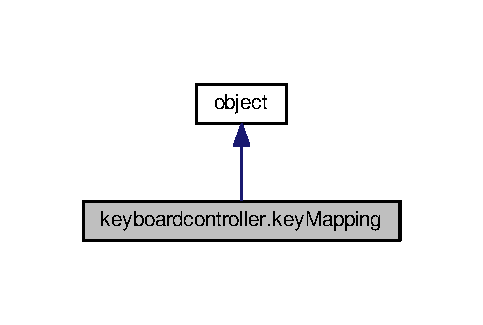
\includegraphics[width=232pt]{classkeyboardcontroller_1_1keyMapping__inherit__graph}
\end{center}
\end{figure}


Collaboration diagram for keyboardcontroller.\-key\-Mapping\-:
\nopagebreak
\begin{figure}[H]
\begin{center}
\leavevmode
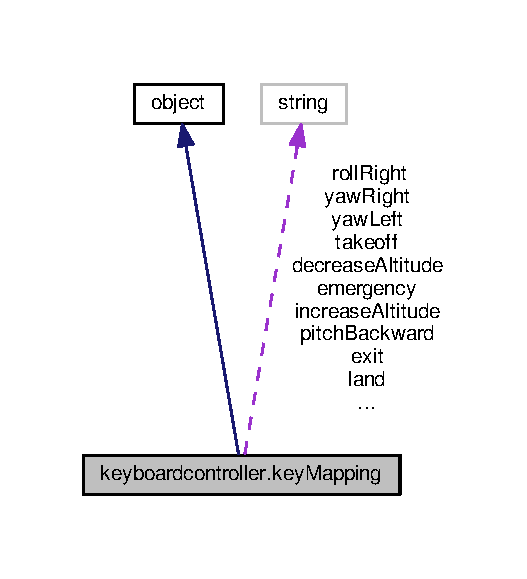
\includegraphics[width=232pt]{classkeyboardcontroller_1_1keyMapping__coll__graph}
\end{center}
\end{figure}


The documentation for this class was generated from the following file\-:\begin{DoxyCompactItemize}
\item 
keyboardcontroller.\-py\end{DoxyCompactItemize}

\hypertarget{classclusterClass_1_1Point}{\section{cluster\-Class.\-Point Class Reference}
\label{classclusterClass_1_1Point}\index{cluster\-Class.\-Point@{cluster\-Class.\-Point}}
}


The documentation for this class was generated from the following file\-:\begin{DoxyCompactItemize}
\item 
cluster\-Class.\-py\end{DoxyCompactItemize}

\hypertarget{classtarget__marker_1_1rvizMarkers}{\section{target\-\_\-marker.\-rviz\-Markers Class Reference}
\label{classtarget__marker_1_1rvizMarkers}\index{target\-\_\-marker.\-rviz\-Markers@{target\-\_\-marker.\-rviz\-Markers}}
}


Inheritance diagram for target\-\_\-marker.\-rviz\-Markers\-:
\nopagebreak
\begin{figure}[H]
\begin{center}
\leavevmode
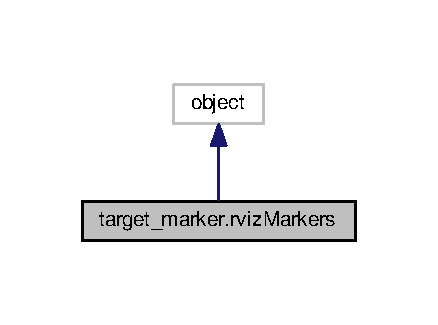
\includegraphics[width=210pt]{classtarget__marker_1_1rvizMarkers__inherit__graph}
\end{center}
\end{figure}


Collaboration diagram for target\-\_\-marker.\-rviz\-Markers\-:
\nopagebreak
\begin{figure}[H]
\begin{center}
\leavevmode
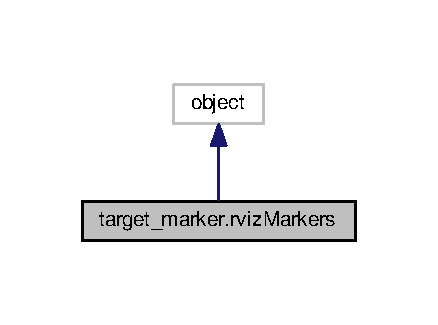
\includegraphics[width=210pt]{classtarget__marker_1_1rvizMarkers__coll__graph}
\end{center}
\end{figure}


The documentation for this class was generated from the following file\-:\begin{DoxyCompactItemize}
\item 
target\-\_\-marker.\-py\end{DoxyCompactItemize}

\hypertarget{classstaircaseai_1_1staircaseAI}{\section{staircaseai.\-staircase\-A\-I Class Reference}
\label{classstaircaseai_1_1staircaseAI}\index{staircaseai.\-staircase\-A\-I@{staircaseai.\-staircase\-A\-I}}
}


Collaboration diagram for staircaseai.\-staircase\-A\-I\-:
\nopagebreak
\begin{figure}[H]
\begin{center}
\leavevmode
\includegraphics[width=263pt]{classstaircaseai_1_1staircaseAI__coll__graph}
\end{center}
\end{figure}
\subsection*{Public Member Functions}
\begin{DoxyCompactItemize}
\item 
def \hyperlink{classstaircaseai_1_1staircaseAI_a959826fb3658b9e4080fdad1af3db9e0}{\-\_\-\-\_\-init\-\_\-\-\_\-}
\begin{DoxyCompactList}\small\item\em Initialize the A\-I class. \end{DoxyCompactList}\item 
def \hyperlink{classstaircaseai_1_1staircaseAI_a4ff981aeb976bec76974ff49782cc84b}{log}
\begin{DoxyCompactList}\small\item\em Puts text in the logscreen of the A\-I G\-U\-I. \end{DoxyCompactList}\item 
def \hyperlink{classstaircaseai_1_1staircaseAI_a53c80e974fec7df7ce206eeff7e44d26}{log\-Det}
\begin{DoxyCompactList}\small\item\em Puts text in the logscreen of the A\-I G\-U\-I. \end{DoxyCompactList}\item 
def \hyperlink{classstaircaseai_1_1staircaseAI_a7170e090765a0c5664664108e3f38ea1}{launch\-R\-V\-I\-Z}
\begin{DoxyCompactList}\small\item\em Launch rviz with the custom setup that is used in ardrone\-\_\-controller together with launch\-Static\-Tf() \end{DoxyCompactList}\item 
def \hyperlink{classstaircaseai_1_1staircaseAI_a0b234cbac093233518729fa5ea0ad725}{launch\-Detection\-Node}
\begin{DoxyCompactList}\small\item\em Launch pointcloudregistration with all its related nodes\-: Static T\-F transform, Image Rectifier and L\-S\-D\-\_\-\-S\-L\-A\-M. \end{DoxyCompactList}\item 
def \hyperlink{classstaircaseai_1_1staircaseAI_a5274e2c215ae921ba6f299639215588b}{launch\-Ardrone\-Driver}
\item 
def \hyperlink{classstaircaseai_1_1staircaseAI_ad6c9232a0f6421ddbedf68b45bda1fe6}{launch\-Tum\-Ardrone}
\item 
def \hyperlink{classstaircaseai_1_1staircaseAI_acef3807e16c5df0f1d4723c33785f72e}{launch\-L\-S\-D\-S\-L\-A\-M\-Viewer}
\item 
def \hyperlink{classstaircaseai_1_1staircaseAI_a72d9ae05f9b3a8ac4b937e284164d5c5}{launchrqt\-Image\-Viewer}
\item 
def \hyperlink{classstaircaseai_1_1staircaseAI_a0e7b18b6a8d981ee6156ac1d3bc05485}{send\-Command}
\item 
def \hyperlink{classstaircaseai_1_1staircaseAI_a7321e77bc12492d99fb34ff729fb29c2}{goto\-Origin}
\item 
def \hyperlink{classstaircaseai_1_1staircaseAI_adf368404f5be7a0f97a858d620000456}{stop\-A\-I}
\item 
def \hyperlink{classstaircaseai_1_1staircaseAI_a1a4d524a29a3fbe6151151b42beede65}{go\-A\-I}
\item 
def \hyperlink{classstaircaseai_1_1staircaseAI_a4a69816800ed71ce87bd49427e5106e5}{reset\-E\-K\-F}
\item 
def \hyperlink{classstaircaseai_1_1staircaseAI_a0018cc957508941977beb292aa38e660}{reset\-P\-T\-A\-M}
\item 
def \hyperlink{classstaircaseai_1_1staircaseAI_a4c6f190b346d73401b6a93e1f6018565}{reset\-L\-S\-D\-S\-L\-A\-M}
\item 
def \hyperlink{classstaircaseai_1_1staircaseAI_aab2dc561edc8cb7b6575ce6a82fa19d4}{init\-L\-S\-D\-S\-L\-A\-M}
\item 
def \hyperlink{classstaircaseai_1_1staircaseAI_ad23031b5507a48abfbfea19671cf73ca}{initialize\-A\-I}
\item 
def \hyperlink{classstaircaseai_1_1staircaseAI_a0d82ca122f05000e0192e5f6e4810e43}{takeoff}
\item 
def \hyperlink{classstaircaseai_1_1staircaseAI_ace7a55f711f5fb559531fe5f6a1ea61f}{close}
\begin{DoxyCompactList}\small\item\em Close the A\-I G\-U\-I interface. \end{DoxyCompactList}\end{DoxyCompactItemize}
\subsection*{Public Attributes}
\begin{DoxyCompactItemize}
\item 
\hyperlink{classstaircaseai_1_1staircaseAI_a95e3078cae642f3569ea7ea043cddc3f}{window}
\item 
\hyperlink{classstaircaseai_1_1staircaseAI_a4fe728ac07ff17300ede98396d4516dc}{log\-Text}
\item 
\hyperlink{classstaircaseai_1_1staircaseAI_a69f3626f7e9a387ecf066fc874fb9b15}{detection\-Text}
\item 
\hyperlink{classstaircaseai_1_1staircaseAI_a1f55704fa569f33c5cabd6e89c549dc6}{target\-Locked\-Text}
\item 
\hyperlink{classstaircaseai_1_1staircaseAI_aae321ff5a9a1cffe907c562ba4c6b39f}{controller}
\item 
\hyperlink{classstaircaseai_1_1staircaseAI_a94eefb2cb8d38235945f714fe35b2e5b}{detection\-Marker\-Publisher}
\item 
\hyperlink{classstaircaseai_1_1staircaseAI_ae21365d23660c43e89c13ef633c7fe65}{goal\-Marker\-Publisher}
\item 
\hyperlink{classstaircaseai_1_1staircaseAI_a84126efb40c0a7d59dff2b930ec0a63c}{tum\-Com\-Publisher}
\item 
\hyperlink{classstaircaseai_1_1staircaseAI_ad4b23f2ca76299504bf0ed5492293b10}{cluster}
\item 
\hyperlink{classstaircaseai_1_1staircaseAI_aa94cc788015f2cf55e5e0755b95341fe}{target\-Sub}
\item 
\hyperlink{classstaircaseai_1_1staircaseAI_a2c20eaa6e814025adfe71f11737dd0cf}{command\-Entry\-Text}
\item 
\hyperlink{classstaircaseai_1_1staircaseAI_abe6ce43882cbd5e478493177450c9023}{ardrone\-Driver\-Lbl}
\item 
\hyperlink{classstaircaseai_1_1staircaseAI_a6b07562110670bd39dfaa76c3d289f4c}{tum\-Ardrone\-Lbl}
\item 
\hyperlink{classstaircaseai_1_1staircaseAI_ab2a668e0ee4a8c8eed4982275a34b9f8}{detection\-Node\-Lbl}
\item 
\hyperlink{classstaircaseai_1_1staircaseAI_ae050ef3b610f1f90003f74c89c6562c2}{R\-V\-I\-Z\-Lbl}
\item 
\hyperlink{classstaircaseai_1_1staircaseAI_a027e1496f0f3ecf7be88e2d3986f5bd2}{L\-S\-D\-S\-L\-A\-M\-Viewer\-Lbl}
\item 
\hyperlink{classstaircaseai_1_1staircaseAI_a40b886c5b0bd0895901671e0bdc1a006}{rqt\-Image\-Viewer\-Lbl}
\item 
\hyperlink{classstaircaseai_1_1staircaseAI_a833c982cff34fb60a0fb6f66f80efb25}{launcher}
\item 
\hyperlink{classstaircaseai_1_1staircaseAI_ac9966f9d12d8d3e73f0c5ac6891243c6}{R\-V\-I\-Z\-Status}
\item 
\hyperlink{classstaircaseai_1_1staircaseAI_a54bcc18605f2331eeb8d42a0709b3590}{R\-V\-I\-Z\-Process}
\item 
\hyperlink{classstaircaseai_1_1staircaseAI_ad3fdf6d0b4f17644da041f09e15b3ca7}{detection\-Node\-Status}
\item 
\hyperlink{classstaircaseai_1_1staircaseAI_a01c439ebe7570405bb22f82ba5a0bb3e}{static\-Tf\-Process}
\item 
\hyperlink{classstaircaseai_1_1staircaseAI_a77b90c85075237529ae93835fd2af2bd}{image\-Rectify\-Process}
\item 
\hyperlink{classstaircaseai_1_1staircaseAI_a5e60775b7acf386fc10cb0ef2f118bc8}{lsdslam\-Process}
\item 
\hyperlink{classstaircaseai_1_1staircaseAI_a87462cc129cb86ab0aaef5b8731cba6c}{detection\-Process}
\item 
\hyperlink{classstaircaseai_1_1staircaseAI_a2f76e2a18d929a8d80ed7d8090e3884a}{ardrone\-Driver\-Status}
\item 
\hyperlink{classstaircaseai_1_1staircaseAI_a1dcc49f394aa217782d18a252c095d91}{ardrone\-Driver\-Process}
\item 
\hyperlink{classstaircaseai_1_1staircaseAI_af27dfa875e03ac7646b25a655318e7e6}{tum\-Ardrone\-Status}
\item 
\hyperlink{classstaircaseai_1_1staircaseAI_a7e495d7bf55a5c90c7b6c342d93e3f58}{drone\-Stateestimation\-Process}
\item 
\hyperlink{classstaircaseai_1_1staircaseAI_a40cdd3e980ae70333a716ceb08dde2bf}{drone\-Autopilot\-Process}
\item 
\hyperlink{classstaircaseai_1_1staircaseAI_ac4392e3c93f4aedf23195b659ccef0c1}{drone\-Gui\-Process}
\item 
\hyperlink{classstaircaseai_1_1staircaseAI_ae6980c88f11e387fec4f4558e1fd60ec}{L\-S\-D\-S\-L\-A\-M\-Viewer\-Status}
\item 
\hyperlink{classstaircaseai_1_1staircaseAI_ac0e22a971bbe5e53dc1e085f7d4053b4}{L\-S\-D\-S\-L\-A\-M\-Viewer\-Process}
\item 
\hyperlink{classstaircaseai_1_1staircaseAI_a3bf21dbce86df4212e2a71d8449acfd3}{rqt\-Image\-Viewer\-Status}
\item 
\hyperlink{classstaircaseai_1_1staircaseAI_a6d00dba2967e83eb5114c61381a1db29}{rqt\-Image\-Viewer\-Process}
\end{DoxyCompactItemize}
\subsection*{Static Public Attributes}
\begin{DoxyCompactItemize}
\item 
string \hyperlink{classstaircaseai_1_1staircaseAI_a5eacd7c55a1736b84c4d08031c9c8dbc}{I\-D} = \char`\"{}A\-I\char`\"{}
\item 
int \hyperlink{classstaircaseai_1_1staircaseAI_a81113025f948e62b7d85719ddd1cc189}{ardrone\-Driver\-Status} = 0
\item 
int \hyperlink{classstaircaseai_1_1staircaseAI_a94e2925e1c0eca37cbdbfc7201dabcb6}{tum\-Ardrone\-Status} = 0
\item 
int \hyperlink{classstaircaseai_1_1staircaseAI_af1b341a22ebf3a672a1168cb7bed7a18}{detection\-Node\-Status} = 0
\item 
int \hyperlink{classstaircaseai_1_1staircaseAI_add2effa5e0e73d315ac2fc563c4370af}{R\-V\-I\-Z\-Status} = 0
\item 
int \hyperlink{classstaircaseai_1_1staircaseAI_a0ba4e3d2088a3c69b7afc3cdc40986c4}{L\-S\-D\-S\-L\-A\-M\-Viewer\-Status} = 0
\item 
int \hyperlink{classstaircaseai_1_1staircaseAI_a1480f7f7d21ef55eac0d17876b33de1b}{rqt\-Image\-Viewer\-Status} = 0
\end{DoxyCompactItemize}


\subsection{Detailed Description}


Definition at line 11 of file staircaseai.\-py.



\subsection{Constructor \& Destructor Documentation}
\hypertarget{classstaircaseai_1_1staircaseAI_a959826fb3658b9e4080fdad1af3db9e0}{\index{staircaseai\-::staircase\-A\-I@{staircaseai\-::staircase\-A\-I}!\-\_\-\-\_\-init\-\_\-\-\_\-@{\-\_\-\-\_\-init\-\_\-\-\_\-}}
\index{\-\_\-\-\_\-init\-\_\-\-\_\-@{\-\_\-\-\_\-init\-\_\-\-\_\-}!staircaseai::staircaseAI@{staircaseai\-::staircase\-A\-I}}
\subsubsection[{\-\_\-\-\_\-init\-\_\-\-\_\-}]{\setlength{\rightskip}{0pt plus 5cm}def staircaseai.\-staircase\-A\-I.\-\_\-\-\_\-init\-\_\-\-\_\- (
\begin{DoxyParamCaption}
\item[{}]{self, }
\item[{}]{master, }
\item[{}]{C\-O\-N\-T\-R\-O\-L\-L\-E\-R}
\end{DoxyParamCaption}
)}}\label{classstaircaseai_1_1staircaseAI_a959826fb3658b9e4080fdad1af3db9e0}


Initialize the A\-I class. 



Definition at line 23 of file staircaseai.\-py.



\subsection{Member Function Documentation}
\hypertarget{classstaircaseai_1_1staircaseAI_ace7a55f711f5fb559531fe5f6a1ea61f}{\index{staircaseai\-::staircase\-A\-I@{staircaseai\-::staircase\-A\-I}!close@{close}}
\index{close@{close}!staircaseai::staircaseAI@{staircaseai\-::staircase\-A\-I}}
\subsubsection[{close}]{\setlength{\rightskip}{0pt plus 5cm}def staircaseai.\-staircase\-A\-I.\-close (
\begin{DoxyParamCaption}
\item[{}]{self}
\end{DoxyParamCaption}
)}}\label{classstaircaseai_1_1staircaseAI_ace7a55f711f5fb559531fe5f6a1ea61f}


Close the A\-I G\-U\-I interface. 



Definition at line 377 of file staircaseai.\-py.

\hypertarget{classstaircaseai_1_1staircaseAI_a1a4d524a29a3fbe6151151b42beede65}{\index{staircaseai\-::staircase\-A\-I@{staircaseai\-::staircase\-A\-I}!go\-A\-I@{go\-A\-I}}
\index{go\-A\-I@{go\-A\-I}!staircaseai::staircaseAI@{staircaseai\-::staircase\-A\-I}}
\subsubsection[{go\-A\-I}]{\setlength{\rightskip}{0pt plus 5cm}def staircaseai.\-staircase\-A\-I.\-go\-A\-I (
\begin{DoxyParamCaption}
\item[{}]{self}
\end{DoxyParamCaption}
)}}\label{classstaircaseai_1_1staircaseAI_a1a4d524a29a3fbe6151151b42beede65}


Definition at line 312 of file staircaseai.\-py.

\hypertarget{classstaircaseai_1_1staircaseAI_a7321e77bc12492d99fb34ff729fb29c2}{\index{staircaseai\-::staircase\-A\-I@{staircaseai\-::staircase\-A\-I}!goto\-Origin@{goto\-Origin}}
\index{goto\-Origin@{goto\-Origin}!staircaseai::staircaseAI@{staircaseai\-::staircase\-A\-I}}
\subsubsection[{goto\-Origin}]{\setlength{\rightskip}{0pt plus 5cm}def staircaseai.\-staircase\-A\-I.\-goto\-Origin (
\begin{DoxyParamCaption}
\item[{}]{self}
\end{DoxyParamCaption}
)}}\label{classstaircaseai_1_1staircaseAI_a7321e77bc12492d99fb34ff729fb29c2}


Definition at line 303 of file staircaseai.\-py.

\hypertarget{classstaircaseai_1_1staircaseAI_ad23031b5507a48abfbfea19671cf73ca}{\index{staircaseai\-::staircase\-A\-I@{staircaseai\-::staircase\-A\-I}!initialize\-A\-I@{initialize\-A\-I}}
\index{initialize\-A\-I@{initialize\-A\-I}!staircaseai::staircaseAI@{staircaseai\-::staircase\-A\-I}}
\subsubsection[{initialize\-A\-I}]{\setlength{\rightskip}{0pt plus 5cm}def staircaseai.\-staircase\-A\-I.\-initialize\-A\-I (
\begin{DoxyParamCaption}
\item[{}]{self}
\end{DoxyParamCaption}
)}}\label{classstaircaseai_1_1staircaseAI_ad23031b5507a48abfbfea19671cf73ca}


Definition at line 346 of file staircaseai.\-py.

\hypertarget{classstaircaseai_1_1staircaseAI_aab2dc561edc8cb7b6575ce6a82fa19d4}{\index{staircaseai\-::staircase\-A\-I@{staircaseai\-::staircase\-A\-I}!init\-L\-S\-D\-S\-L\-A\-M@{init\-L\-S\-D\-S\-L\-A\-M}}
\index{init\-L\-S\-D\-S\-L\-A\-M@{init\-L\-S\-D\-S\-L\-A\-M}!staircaseai::staircaseAI@{staircaseai\-::staircase\-A\-I}}
\subsubsection[{init\-L\-S\-D\-S\-L\-A\-M}]{\setlength{\rightskip}{0pt plus 5cm}def staircaseai.\-staircase\-A\-I.\-init\-L\-S\-D\-S\-L\-A\-M (
\begin{DoxyParamCaption}
\item[{}]{self}
\end{DoxyParamCaption}
)}}\label{classstaircaseai_1_1staircaseAI_aab2dc561edc8cb7b6575ce6a82fa19d4}


Definition at line 343 of file staircaseai.\-py.

\hypertarget{classstaircaseai_1_1staircaseAI_a5274e2c215ae921ba6f299639215588b}{\index{staircaseai\-::staircase\-A\-I@{staircaseai\-::staircase\-A\-I}!launch\-Ardrone\-Driver@{launch\-Ardrone\-Driver}}
\index{launch\-Ardrone\-Driver@{launch\-Ardrone\-Driver}!staircaseai::staircaseAI@{staircaseai\-::staircase\-A\-I}}
\subsubsection[{launch\-Ardrone\-Driver}]{\setlength{\rightskip}{0pt plus 5cm}def staircaseai.\-staircase\-A\-I.\-launch\-Ardrone\-Driver (
\begin{DoxyParamCaption}
\item[{}]{self}
\end{DoxyParamCaption}
)}}\label{classstaircaseai_1_1staircaseAI_a5274e2c215ae921ba6f299639215588b}


Definition at line 239 of file staircaseai.\-py.

\hypertarget{classstaircaseai_1_1staircaseAI_a0b234cbac093233518729fa5ea0ad725}{\index{staircaseai\-::staircase\-A\-I@{staircaseai\-::staircase\-A\-I}!launch\-Detection\-Node@{launch\-Detection\-Node}}
\index{launch\-Detection\-Node@{launch\-Detection\-Node}!staircaseai::staircaseAI@{staircaseai\-::staircase\-A\-I}}
\subsubsection[{launch\-Detection\-Node}]{\setlength{\rightskip}{0pt plus 5cm}def staircaseai.\-staircase\-A\-I.\-launch\-Detection\-Node (
\begin{DoxyParamCaption}
\item[{}]{self}
\end{DoxyParamCaption}
)}}\label{classstaircaseai_1_1staircaseAI_a0b234cbac093233518729fa5ea0ad725}


Launch pointcloudregistration with all its related nodes\-: Static T\-F transform, Image Rectifier and L\-S\-D\-\_\-\-S\-L\-A\-M. 



Definition at line 205 of file staircaseai.\-py.

\hypertarget{classstaircaseai_1_1staircaseAI_acef3807e16c5df0f1d4723c33785f72e}{\index{staircaseai\-::staircase\-A\-I@{staircaseai\-::staircase\-A\-I}!launch\-L\-S\-D\-S\-L\-A\-M\-Viewer@{launch\-L\-S\-D\-S\-L\-A\-M\-Viewer}}
\index{launch\-L\-S\-D\-S\-L\-A\-M\-Viewer@{launch\-L\-S\-D\-S\-L\-A\-M\-Viewer}!staircaseai::staircaseAI@{staircaseai\-::staircase\-A\-I}}
\subsubsection[{launch\-L\-S\-D\-S\-L\-A\-M\-Viewer}]{\setlength{\rightskip}{0pt plus 5cm}def staircaseai.\-staircase\-A\-I.\-launch\-L\-S\-D\-S\-L\-A\-M\-Viewer (
\begin{DoxyParamCaption}
\item[{}]{self}
\end{DoxyParamCaption}
)}}\label{classstaircaseai_1_1staircaseAI_acef3807e16c5df0f1d4723c33785f72e}


Definition at line 274 of file staircaseai.\-py.

\hypertarget{classstaircaseai_1_1staircaseAI_a72d9ae05f9b3a8ac4b937e284164d5c5}{\index{staircaseai\-::staircase\-A\-I@{staircaseai\-::staircase\-A\-I}!launchrqt\-Image\-Viewer@{launchrqt\-Image\-Viewer}}
\index{launchrqt\-Image\-Viewer@{launchrqt\-Image\-Viewer}!staircaseai::staircaseAI@{staircaseai\-::staircase\-A\-I}}
\subsubsection[{launchrqt\-Image\-Viewer}]{\setlength{\rightskip}{0pt plus 5cm}def staircaseai.\-staircase\-A\-I.\-launchrqt\-Image\-Viewer (
\begin{DoxyParamCaption}
\item[{}]{self}
\end{DoxyParamCaption}
)}}\label{classstaircaseai_1_1staircaseAI_a72d9ae05f9b3a8ac4b937e284164d5c5}


Definition at line 286 of file staircaseai.\-py.

\hypertarget{classstaircaseai_1_1staircaseAI_a7170e090765a0c5664664108e3f38ea1}{\index{staircaseai\-::staircase\-A\-I@{staircaseai\-::staircase\-A\-I}!launch\-R\-V\-I\-Z@{launch\-R\-V\-I\-Z}}
\index{launch\-R\-V\-I\-Z@{launch\-R\-V\-I\-Z}!staircaseai::staircaseAI@{staircaseai\-::staircase\-A\-I}}
\subsubsection[{launch\-R\-V\-I\-Z}]{\setlength{\rightskip}{0pt plus 5cm}def staircaseai.\-staircase\-A\-I.\-launch\-R\-V\-I\-Z (
\begin{DoxyParamCaption}
\item[{}]{self}
\end{DoxyParamCaption}
)}}\label{classstaircaseai_1_1staircaseAI_a7170e090765a0c5664664108e3f38ea1}


Launch rviz with the custom setup that is used in ardrone\-\_\-controller together with launch\-Static\-Tf() 



Definition at line 187 of file staircaseai.\-py.

\hypertarget{classstaircaseai_1_1staircaseAI_ad6c9232a0f6421ddbedf68b45bda1fe6}{\index{staircaseai\-::staircase\-A\-I@{staircaseai\-::staircase\-A\-I}!launch\-Tum\-Ardrone@{launch\-Tum\-Ardrone}}
\index{launch\-Tum\-Ardrone@{launch\-Tum\-Ardrone}!staircaseai::staircaseAI@{staircaseai\-::staircase\-A\-I}}
\subsubsection[{launch\-Tum\-Ardrone}]{\setlength{\rightskip}{0pt plus 5cm}def staircaseai.\-staircase\-A\-I.\-launch\-Tum\-Ardrone (
\begin{DoxyParamCaption}
\item[{}]{self}
\end{DoxyParamCaption}
)}}\label{classstaircaseai_1_1staircaseAI_ad6c9232a0f6421ddbedf68b45bda1fe6}


Definition at line 256 of file staircaseai.\-py.

\hypertarget{classstaircaseai_1_1staircaseAI_a4ff981aeb976bec76974ff49782cc84b}{\index{staircaseai\-::staircase\-A\-I@{staircaseai\-::staircase\-A\-I}!log@{log}}
\index{log@{log}!staircaseai::staircaseAI@{staircaseai\-::staircase\-A\-I}}
\subsubsection[{log}]{\setlength{\rightskip}{0pt plus 5cm}def staircaseai.\-staircase\-A\-I.\-log (
\begin{DoxyParamCaption}
\item[{}]{self, }
\item[{}]{string}
\end{DoxyParamCaption}
)}}\label{classstaircaseai_1_1staircaseAI_a4ff981aeb976bec76974ff49782cc84b}


Puts text in the logscreen of the A\-I G\-U\-I. 



Definition at line 176 of file staircaseai.\-py.

\hypertarget{classstaircaseai_1_1staircaseAI_a53c80e974fec7df7ce206eeff7e44d26}{\index{staircaseai\-::staircase\-A\-I@{staircaseai\-::staircase\-A\-I}!log\-Det@{log\-Det}}
\index{log\-Det@{log\-Det}!staircaseai::staircaseAI@{staircaseai\-::staircase\-A\-I}}
\subsubsection[{log\-Det}]{\setlength{\rightskip}{0pt plus 5cm}def staircaseai.\-staircase\-A\-I.\-log\-Det (
\begin{DoxyParamCaption}
\item[{}]{self, }
\item[{}]{string}
\end{DoxyParamCaption}
)}}\label{classstaircaseai_1_1staircaseAI_a53c80e974fec7df7ce206eeff7e44d26}


Puts text in the logscreen of the A\-I G\-U\-I. 



Definition at line 181 of file staircaseai.\-py.

\hypertarget{classstaircaseai_1_1staircaseAI_a4a69816800ed71ce87bd49427e5106e5}{\index{staircaseai\-::staircase\-A\-I@{staircaseai\-::staircase\-A\-I}!reset\-E\-K\-F@{reset\-E\-K\-F}}
\index{reset\-E\-K\-F@{reset\-E\-K\-F}!staircaseai::staircaseAI@{staircaseai\-::staircase\-A\-I}}
\subsubsection[{reset\-E\-K\-F}]{\setlength{\rightskip}{0pt plus 5cm}def staircaseai.\-staircase\-A\-I.\-reset\-E\-K\-F (
\begin{DoxyParamCaption}
\item[{}]{self}
\end{DoxyParamCaption}
)}}\label{classstaircaseai_1_1staircaseAI_a4a69816800ed71ce87bd49427e5106e5}


Definition at line 322 of file staircaseai.\-py.

\hypertarget{classstaircaseai_1_1staircaseAI_a4c6f190b346d73401b6a93e1f6018565}{\index{staircaseai\-::staircase\-A\-I@{staircaseai\-::staircase\-A\-I}!reset\-L\-S\-D\-S\-L\-A\-M@{reset\-L\-S\-D\-S\-L\-A\-M}}
\index{reset\-L\-S\-D\-S\-L\-A\-M@{reset\-L\-S\-D\-S\-L\-A\-M}!staircaseai::staircaseAI@{staircaseai\-::staircase\-A\-I}}
\subsubsection[{reset\-L\-S\-D\-S\-L\-A\-M}]{\setlength{\rightskip}{0pt plus 5cm}def staircaseai.\-staircase\-A\-I.\-reset\-L\-S\-D\-S\-L\-A\-M (
\begin{DoxyParamCaption}
\item[{}]{self}
\end{DoxyParamCaption}
)}}\label{classstaircaseai_1_1staircaseAI_a4c6f190b346d73401b6a93e1f6018565}


Definition at line 334 of file staircaseai.\-py.

\hypertarget{classstaircaseai_1_1staircaseAI_a0018cc957508941977beb292aa38e660}{\index{staircaseai\-::staircase\-A\-I@{staircaseai\-::staircase\-A\-I}!reset\-P\-T\-A\-M@{reset\-P\-T\-A\-M}}
\index{reset\-P\-T\-A\-M@{reset\-P\-T\-A\-M}!staircaseai::staircaseAI@{staircaseai\-::staircase\-A\-I}}
\subsubsection[{reset\-P\-T\-A\-M}]{\setlength{\rightskip}{0pt plus 5cm}def staircaseai.\-staircase\-A\-I.\-reset\-P\-T\-A\-M (
\begin{DoxyParamCaption}
\item[{}]{self}
\end{DoxyParamCaption}
)}}\label{classstaircaseai_1_1staircaseAI_a0018cc957508941977beb292aa38e660}


Definition at line 329 of file staircaseai.\-py.

\hypertarget{classstaircaseai_1_1staircaseAI_a0e7b18b6a8d981ee6156ac1d3bc05485}{\index{staircaseai\-::staircase\-A\-I@{staircaseai\-::staircase\-A\-I}!send\-Command@{send\-Command}}
\index{send\-Command@{send\-Command}!staircaseai::staircaseAI@{staircaseai\-::staircase\-A\-I}}
\subsubsection[{send\-Command}]{\setlength{\rightskip}{0pt plus 5cm}def staircaseai.\-staircase\-A\-I.\-send\-Command (
\begin{DoxyParamCaption}
\item[{}]{self}
\end{DoxyParamCaption}
)}}\label{classstaircaseai_1_1staircaseAI_a0e7b18b6a8d981ee6156ac1d3bc05485}


Definition at line 298 of file staircaseai.\-py.

\hypertarget{classstaircaseai_1_1staircaseAI_adf368404f5be7a0f97a858d620000456}{\index{staircaseai\-::staircase\-A\-I@{staircaseai\-::staircase\-A\-I}!stop\-A\-I@{stop\-A\-I}}
\index{stop\-A\-I@{stop\-A\-I}!staircaseai::staircaseAI@{staircaseai\-::staircase\-A\-I}}
\subsubsection[{stop\-A\-I}]{\setlength{\rightskip}{0pt plus 5cm}def staircaseai.\-staircase\-A\-I.\-stop\-A\-I (
\begin{DoxyParamCaption}
\item[{}]{self}
\end{DoxyParamCaption}
)}}\label{classstaircaseai_1_1staircaseAI_adf368404f5be7a0f97a858d620000456}


Definition at line 308 of file staircaseai.\-py.

\hypertarget{classstaircaseai_1_1staircaseAI_a0d82ca122f05000e0192e5f6e4810e43}{\index{staircaseai\-::staircase\-A\-I@{staircaseai\-::staircase\-A\-I}!takeoff@{takeoff}}
\index{takeoff@{takeoff}!staircaseai::staircaseAI@{staircaseai\-::staircase\-A\-I}}
\subsubsection[{takeoff}]{\setlength{\rightskip}{0pt plus 5cm}def staircaseai.\-staircase\-A\-I.\-takeoff (
\begin{DoxyParamCaption}
\item[{}]{self}
\end{DoxyParamCaption}
)}}\label{classstaircaseai_1_1staircaseAI_a0d82ca122f05000e0192e5f6e4810e43}


Definition at line 371 of file staircaseai.\-py.



\subsection{Member Data Documentation}
\hypertarget{classstaircaseai_1_1staircaseAI_abe6ce43882cbd5e478493177450c9023}{\index{staircaseai\-::staircase\-A\-I@{staircaseai\-::staircase\-A\-I}!ardrone\-Driver\-Lbl@{ardrone\-Driver\-Lbl}}
\index{ardrone\-Driver\-Lbl@{ardrone\-Driver\-Lbl}!staircaseai::staircaseAI@{staircaseai\-::staircase\-A\-I}}
\subsubsection[{ardrone\-Driver\-Lbl}]{\setlength{\rightskip}{0pt plus 5cm}staircaseai.\-staircase\-A\-I.\-ardrone\-Driver\-Lbl}}\label{classstaircaseai_1_1staircaseAI_abe6ce43882cbd5e478493177450c9023}


Definition at line 93 of file staircaseai.\-py.

\hypertarget{classstaircaseai_1_1staircaseAI_a1dcc49f394aa217782d18a252c095d91}{\index{staircaseai\-::staircase\-A\-I@{staircaseai\-::staircase\-A\-I}!ardrone\-Driver\-Process@{ardrone\-Driver\-Process}}
\index{ardrone\-Driver\-Process@{ardrone\-Driver\-Process}!staircaseai::staircaseAI@{staircaseai\-::staircase\-A\-I}}
\subsubsection[{ardrone\-Driver\-Process}]{\setlength{\rightskip}{0pt plus 5cm}staircaseai.\-staircase\-A\-I.\-ardrone\-Driver\-Process}}\label{classstaircaseai_1_1staircaseAI_a1dcc49f394aa217782d18a252c095d91}


Definition at line 248 of file staircaseai.\-py.

\hypertarget{classstaircaseai_1_1staircaseAI_a81113025f948e62b7d85719ddd1cc189}{\index{staircaseai\-::staircase\-A\-I@{staircaseai\-::staircase\-A\-I}!ardrone\-Driver\-Status@{ardrone\-Driver\-Status}}
\index{ardrone\-Driver\-Status@{ardrone\-Driver\-Status}!staircaseai::staircaseAI@{staircaseai\-::staircase\-A\-I}}
\subsubsection[{ardrone\-Driver\-Status}]{\setlength{\rightskip}{0pt plus 5cm}int staircaseai.\-staircase\-A\-I.\-ardrone\-Driver\-Status = 0\hspace{0.3cm}{\ttfamily [static]}}}\label{classstaircaseai_1_1staircaseAI_a81113025f948e62b7d85719ddd1cc189}


Definition at line 14 of file staircaseai.\-py.

\hypertarget{classstaircaseai_1_1staircaseAI_a2f76e2a18d929a8d80ed7d8090e3884a}{\index{staircaseai\-::staircase\-A\-I@{staircaseai\-::staircase\-A\-I}!ardrone\-Driver\-Status@{ardrone\-Driver\-Status}}
\index{ardrone\-Driver\-Status@{ardrone\-Driver\-Status}!staircaseai::staircaseAI@{staircaseai\-::staircase\-A\-I}}
\subsubsection[{ardrone\-Driver\-Status}]{\setlength{\rightskip}{0pt plus 5cm}staircaseai.\-staircase\-A\-I.\-ardrone\-Driver\-Status}}\label{classstaircaseai_1_1staircaseAI_a2f76e2a18d929a8d80ed7d8090e3884a}


Definition at line 240 of file staircaseai.\-py.

\hypertarget{classstaircaseai_1_1staircaseAI_ad4b23f2ca76299504bf0ed5492293b10}{\index{staircaseai\-::staircase\-A\-I@{staircaseai\-::staircase\-A\-I}!cluster@{cluster}}
\index{cluster@{cluster}!staircaseai::staircaseAI@{staircaseai\-::staircase\-A\-I}}
\subsubsection[{cluster}]{\setlength{\rightskip}{0pt plus 5cm}staircaseai.\-staircase\-A\-I.\-cluster}}\label{classstaircaseai_1_1staircaseAI_ad4b23f2ca76299504bf0ed5492293b10}


Definition at line 57 of file staircaseai.\-py.

\hypertarget{classstaircaseai_1_1staircaseAI_a2c20eaa6e814025adfe71f11737dd0cf}{\index{staircaseai\-::staircase\-A\-I@{staircaseai\-::staircase\-A\-I}!command\-Entry\-Text@{command\-Entry\-Text}}
\index{command\-Entry\-Text@{command\-Entry\-Text}!staircaseai::staircaseAI@{staircaseai\-::staircase\-A\-I}}
\subsubsection[{command\-Entry\-Text}]{\setlength{\rightskip}{0pt plus 5cm}staircaseai.\-staircase\-A\-I.\-command\-Entry\-Text}}\label{classstaircaseai_1_1staircaseAI_a2c20eaa6e814025adfe71f11737dd0cf}


Definition at line 75 of file staircaseai.\-py.

\hypertarget{classstaircaseai_1_1staircaseAI_aae321ff5a9a1cffe907c562ba4c6b39f}{\index{staircaseai\-::staircase\-A\-I@{staircaseai\-::staircase\-A\-I}!controller@{controller}}
\index{controller@{controller}!staircaseai::staircaseAI@{staircaseai\-::staircase\-A\-I}}
\subsubsection[{controller}]{\setlength{\rightskip}{0pt plus 5cm}staircaseai.\-staircase\-A\-I.\-controller}}\label{classstaircaseai_1_1staircaseAI_aae321ff5a9a1cffe907c562ba4c6b39f}


Definition at line 51 of file staircaseai.\-py.

\hypertarget{classstaircaseai_1_1staircaseAI_a94eefb2cb8d38235945f714fe35b2e5b}{\index{staircaseai\-::staircase\-A\-I@{staircaseai\-::staircase\-A\-I}!detection\-Marker\-Publisher@{detection\-Marker\-Publisher}}
\index{detection\-Marker\-Publisher@{detection\-Marker\-Publisher}!staircaseai::staircaseAI@{staircaseai\-::staircase\-A\-I}}
\subsubsection[{detection\-Marker\-Publisher}]{\setlength{\rightskip}{0pt plus 5cm}staircaseai.\-staircase\-A\-I.\-detection\-Marker\-Publisher}}\label{classstaircaseai_1_1staircaseAI_a94eefb2cb8d38235945f714fe35b2e5b}


Definition at line 54 of file staircaseai.\-py.

\hypertarget{classstaircaseai_1_1staircaseAI_ab2a668e0ee4a8c8eed4982275a34b9f8}{\index{staircaseai\-::staircase\-A\-I@{staircaseai\-::staircase\-A\-I}!detection\-Node\-Lbl@{detection\-Node\-Lbl}}
\index{detection\-Node\-Lbl@{detection\-Node\-Lbl}!staircaseai::staircaseAI@{staircaseai\-::staircase\-A\-I}}
\subsubsection[{detection\-Node\-Lbl}]{\setlength{\rightskip}{0pt plus 5cm}staircaseai.\-staircase\-A\-I.\-detection\-Node\-Lbl}}\label{classstaircaseai_1_1staircaseAI_ab2a668e0ee4a8c8eed4982275a34b9f8}


Definition at line 99 of file staircaseai.\-py.

\hypertarget{classstaircaseai_1_1staircaseAI_af1b341a22ebf3a672a1168cb7bed7a18}{\index{staircaseai\-::staircase\-A\-I@{staircaseai\-::staircase\-A\-I}!detection\-Node\-Status@{detection\-Node\-Status}}
\index{detection\-Node\-Status@{detection\-Node\-Status}!staircaseai::staircaseAI@{staircaseai\-::staircase\-A\-I}}
\subsubsection[{detection\-Node\-Status}]{\setlength{\rightskip}{0pt plus 5cm}int staircaseai.\-staircase\-A\-I.\-detection\-Node\-Status = 0\hspace{0.3cm}{\ttfamily [static]}}}\label{classstaircaseai_1_1staircaseAI_af1b341a22ebf3a672a1168cb7bed7a18}


Definition at line 16 of file staircaseai.\-py.

\hypertarget{classstaircaseai_1_1staircaseAI_ad3fdf6d0b4f17644da041f09e15b3ca7}{\index{staircaseai\-::staircase\-A\-I@{staircaseai\-::staircase\-A\-I}!detection\-Node\-Status@{detection\-Node\-Status}}
\index{detection\-Node\-Status@{detection\-Node\-Status}!staircaseai::staircaseAI@{staircaseai\-::staircase\-A\-I}}
\subsubsection[{detection\-Node\-Status}]{\setlength{\rightskip}{0pt plus 5cm}staircaseai.\-staircase\-A\-I.\-detection\-Node\-Status}}\label{classstaircaseai_1_1staircaseAI_ad3fdf6d0b4f17644da041f09e15b3ca7}


Definition at line 206 of file staircaseai.\-py.

\hypertarget{classstaircaseai_1_1staircaseAI_a87462cc129cb86ab0aaef5b8731cba6c}{\index{staircaseai\-::staircase\-A\-I@{staircaseai\-::staircase\-A\-I}!detection\-Process@{detection\-Process}}
\index{detection\-Process@{detection\-Process}!staircaseai::staircaseAI@{staircaseai\-::staircase\-A\-I}}
\subsubsection[{detection\-Process}]{\setlength{\rightskip}{0pt plus 5cm}staircaseai.\-staircase\-A\-I.\-detection\-Process}}\label{classstaircaseai_1_1staircaseAI_a87462cc129cb86ab0aaef5b8731cba6c}


Definition at line 225 of file staircaseai.\-py.

\hypertarget{classstaircaseai_1_1staircaseAI_a69f3626f7e9a387ecf066fc874fb9b15}{\index{staircaseai\-::staircase\-A\-I@{staircaseai\-::staircase\-A\-I}!detection\-Text@{detection\-Text}}
\index{detection\-Text@{detection\-Text}!staircaseai::staircaseAI@{staircaseai\-::staircase\-A\-I}}
\subsubsection[{detection\-Text}]{\setlength{\rightskip}{0pt plus 5cm}staircaseai.\-staircase\-A\-I.\-detection\-Text}}\label{classstaircaseai_1_1staircaseAI_a69f3626f7e9a387ecf066fc874fb9b15}


Definition at line 44 of file staircaseai.\-py.

\hypertarget{classstaircaseai_1_1staircaseAI_a40cdd3e980ae70333a716ceb08dde2bf}{\index{staircaseai\-::staircase\-A\-I@{staircaseai\-::staircase\-A\-I}!drone\-Autopilot\-Process@{drone\-Autopilot\-Process}}
\index{drone\-Autopilot\-Process@{drone\-Autopilot\-Process}!staircaseai::staircaseAI@{staircaseai\-::staircase\-A\-I}}
\subsubsection[{drone\-Autopilot\-Process}]{\setlength{\rightskip}{0pt plus 5cm}staircaseai.\-staircase\-A\-I.\-drone\-Autopilot\-Process}}\label{classstaircaseai_1_1staircaseAI_a40cdd3e980ae70333a716ceb08dde2bf}


Definition at line 262 of file staircaseai.\-py.

\hypertarget{classstaircaseai_1_1staircaseAI_ac4392e3c93f4aedf23195b659ccef0c1}{\index{staircaseai\-::staircase\-A\-I@{staircaseai\-::staircase\-A\-I}!drone\-Gui\-Process@{drone\-Gui\-Process}}
\index{drone\-Gui\-Process@{drone\-Gui\-Process}!staircaseai::staircaseAI@{staircaseai\-::staircase\-A\-I}}
\subsubsection[{drone\-Gui\-Process}]{\setlength{\rightskip}{0pt plus 5cm}staircaseai.\-staircase\-A\-I.\-drone\-Gui\-Process}}\label{classstaircaseai_1_1staircaseAI_ac4392e3c93f4aedf23195b659ccef0c1}


Definition at line 264 of file staircaseai.\-py.

\hypertarget{classstaircaseai_1_1staircaseAI_a7e495d7bf55a5c90c7b6c342d93e3f58}{\index{staircaseai\-::staircase\-A\-I@{staircaseai\-::staircase\-A\-I}!drone\-Stateestimation\-Process@{drone\-Stateestimation\-Process}}
\index{drone\-Stateestimation\-Process@{drone\-Stateestimation\-Process}!staircaseai::staircaseAI@{staircaseai\-::staircase\-A\-I}}
\subsubsection[{drone\-Stateestimation\-Process}]{\setlength{\rightskip}{0pt plus 5cm}staircaseai.\-staircase\-A\-I.\-drone\-Stateestimation\-Process}}\label{classstaircaseai_1_1staircaseAI_a7e495d7bf55a5c90c7b6c342d93e3f58}


Definition at line 260 of file staircaseai.\-py.

\hypertarget{classstaircaseai_1_1staircaseAI_ae21365d23660c43e89c13ef633c7fe65}{\index{staircaseai\-::staircase\-A\-I@{staircaseai\-::staircase\-A\-I}!goal\-Marker\-Publisher@{goal\-Marker\-Publisher}}
\index{goal\-Marker\-Publisher@{goal\-Marker\-Publisher}!staircaseai::staircaseAI@{staircaseai\-::staircase\-A\-I}}
\subsubsection[{goal\-Marker\-Publisher}]{\setlength{\rightskip}{0pt plus 5cm}staircaseai.\-staircase\-A\-I.\-goal\-Marker\-Publisher}}\label{classstaircaseai_1_1staircaseAI_ae21365d23660c43e89c13ef633c7fe65}


Definition at line 55 of file staircaseai.\-py.

\hypertarget{classstaircaseai_1_1staircaseAI_a5eacd7c55a1736b84c4d08031c9c8dbc}{\index{staircaseai\-::staircase\-A\-I@{staircaseai\-::staircase\-A\-I}!I\-D@{I\-D}}
\index{I\-D@{I\-D}!staircaseai::staircaseAI@{staircaseai\-::staircase\-A\-I}}
\subsubsection[{I\-D}]{\setlength{\rightskip}{0pt plus 5cm}string staircaseai.\-staircase\-A\-I.\-I\-D = \char`\"{}A\-I\char`\"{}\hspace{0.3cm}{\ttfamily [static]}}}\label{classstaircaseai_1_1staircaseAI_a5eacd7c55a1736b84c4d08031c9c8dbc}


Definition at line 12 of file staircaseai.\-py.

\hypertarget{classstaircaseai_1_1staircaseAI_a77b90c85075237529ae93835fd2af2bd}{\index{staircaseai\-::staircase\-A\-I@{staircaseai\-::staircase\-A\-I}!image\-Rectify\-Process@{image\-Rectify\-Process}}
\index{image\-Rectify\-Process@{image\-Rectify\-Process}!staircaseai::staircaseAI@{staircaseai\-::staircase\-A\-I}}
\subsubsection[{image\-Rectify\-Process}]{\setlength{\rightskip}{0pt plus 5cm}staircaseai.\-staircase\-A\-I.\-image\-Rectify\-Process}}\label{classstaircaseai_1_1staircaseAI_a77b90c85075237529ae93835fd2af2bd}


Definition at line 212 of file staircaseai.\-py.

\hypertarget{classstaircaseai_1_1staircaseAI_a833c982cff34fb60a0fb6f66f80efb25}{\index{staircaseai\-::staircase\-A\-I@{staircaseai\-::staircase\-A\-I}!launcher@{launcher}}
\index{launcher@{launcher}!staircaseai::staircaseAI@{staircaseai\-::staircase\-A\-I}}
\subsubsection[{launcher}]{\setlength{\rightskip}{0pt plus 5cm}staircaseai.\-staircase\-A\-I.\-launcher}}\label{classstaircaseai_1_1staircaseAI_a833c982cff34fb60a0fb6f66f80efb25}


Definition at line 166 of file staircaseai.\-py.

\hypertarget{classstaircaseai_1_1staircaseAI_a4fe728ac07ff17300ede98396d4516dc}{\index{staircaseai\-::staircase\-A\-I@{staircaseai\-::staircase\-A\-I}!log\-Text@{log\-Text}}
\index{log\-Text@{log\-Text}!staircaseai::staircaseAI@{staircaseai\-::staircase\-A\-I}}
\subsubsection[{log\-Text}]{\setlength{\rightskip}{0pt plus 5cm}staircaseai.\-staircase\-A\-I.\-log\-Text}}\label{classstaircaseai_1_1staircaseAI_a4fe728ac07ff17300ede98396d4516dc}


Definition at line 40 of file staircaseai.\-py.

\hypertarget{classstaircaseai_1_1staircaseAI_a5e60775b7acf386fc10cb0ef2f118bc8}{\index{staircaseai\-::staircase\-A\-I@{staircaseai\-::staircase\-A\-I}!lsdslam\-Process@{lsdslam\-Process}}
\index{lsdslam\-Process@{lsdslam\-Process}!staircaseai::staircaseAI@{staircaseai\-::staircase\-A\-I}}
\subsubsection[{lsdslam\-Process}]{\setlength{\rightskip}{0pt plus 5cm}staircaseai.\-staircase\-A\-I.\-lsdslam\-Process}}\label{classstaircaseai_1_1staircaseAI_a5e60775b7acf386fc10cb0ef2f118bc8}


Definition at line 217 of file staircaseai.\-py.

\hypertarget{classstaircaseai_1_1staircaseAI_a027e1496f0f3ecf7be88e2d3986f5bd2}{\index{staircaseai\-::staircase\-A\-I@{staircaseai\-::staircase\-A\-I}!L\-S\-D\-S\-L\-A\-M\-Viewer\-Lbl@{L\-S\-D\-S\-L\-A\-M\-Viewer\-Lbl}}
\index{L\-S\-D\-S\-L\-A\-M\-Viewer\-Lbl@{L\-S\-D\-S\-L\-A\-M\-Viewer\-Lbl}!staircaseai::staircaseAI@{staircaseai\-::staircase\-A\-I}}
\subsubsection[{L\-S\-D\-S\-L\-A\-M\-Viewer\-Lbl}]{\setlength{\rightskip}{0pt plus 5cm}staircaseai.\-staircase\-A\-I.\-L\-S\-D\-S\-L\-A\-M\-Viewer\-Lbl}}\label{classstaircaseai_1_1staircaseAI_a027e1496f0f3ecf7be88e2d3986f5bd2}


Definition at line 105 of file staircaseai.\-py.

\hypertarget{classstaircaseai_1_1staircaseAI_ac0e22a971bbe5e53dc1e085f7d4053b4}{\index{staircaseai\-::staircase\-A\-I@{staircaseai\-::staircase\-A\-I}!L\-S\-D\-S\-L\-A\-M\-Viewer\-Process@{L\-S\-D\-S\-L\-A\-M\-Viewer\-Process}}
\index{L\-S\-D\-S\-L\-A\-M\-Viewer\-Process@{L\-S\-D\-S\-L\-A\-M\-Viewer\-Process}!staircaseai::staircaseAI@{staircaseai\-::staircase\-A\-I}}
\subsubsection[{L\-S\-D\-S\-L\-A\-M\-Viewer\-Process}]{\setlength{\rightskip}{0pt plus 5cm}staircaseai.\-staircase\-A\-I.\-L\-S\-D\-S\-L\-A\-M\-Viewer\-Process}}\label{classstaircaseai_1_1staircaseAI_ac0e22a971bbe5e53dc1e085f7d4053b4}


Definition at line 278 of file staircaseai.\-py.

\hypertarget{classstaircaseai_1_1staircaseAI_a0ba4e3d2088a3c69b7afc3cdc40986c4}{\index{staircaseai\-::staircase\-A\-I@{staircaseai\-::staircase\-A\-I}!L\-S\-D\-S\-L\-A\-M\-Viewer\-Status@{L\-S\-D\-S\-L\-A\-M\-Viewer\-Status}}
\index{L\-S\-D\-S\-L\-A\-M\-Viewer\-Status@{L\-S\-D\-S\-L\-A\-M\-Viewer\-Status}!staircaseai::staircaseAI@{staircaseai\-::staircase\-A\-I}}
\subsubsection[{L\-S\-D\-S\-L\-A\-M\-Viewer\-Status}]{\setlength{\rightskip}{0pt plus 5cm}int staircaseai.\-staircase\-A\-I.\-L\-S\-D\-S\-L\-A\-M\-Viewer\-Status = 0\hspace{0.3cm}{\ttfamily [static]}}}\label{classstaircaseai_1_1staircaseAI_a0ba4e3d2088a3c69b7afc3cdc40986c4}


Definition at line 18 of file staircaseai.\-py.

\hypertarget{classstaircaseai_1_1staircaseAI_ae6980c88f11e387fec4f4558e1fd60ec}{\index{staircaseai\-::staircase\-A\-I@{staircaseai\-::staircase\-A\-I}!L\-S\-D\-S\-L\-A\-M\-Viewer\-Status@{L\-S\-D\-S\-L\-A\-M\-Viewer\-Status}}
\index{L\-S\-D\-S\-L\-A\-M\-Viewer\-Status@{L\-S\-D\-S\-L\-A\-M\-Viewer\-Status}!staircaseai::staircaseAI@{staircaseai\-::staircase\-A\-I}}
\subsubsection[{L\-S\-D\-S\-L\-A\-M\-Viewer\-Status}]{\setlength{\rightskip}{0pt plus 5cm}staircaseai.\-staircase\-A\-I.\-L\-S\-D\-S\-L\-A\-M\-Viewer\-Status}}\label{classstaircaseai_1_1staircaseAI_ae6980c88f11e387fec4f4558e1fd60ec}


Definition at line 275 of file staircaseai.\-py.

\hypertarget{classstaircaseai_1_1staircaseAI_a40b886c5b0bd0895901671e0bdc1a006}{\index{staircaseai\-::staircase\-A\-I@{staircaseai\-::staircase\-A\-I}!rqt\-Image\-Viewer\-Lbl@{rqt\-Image\-Viewer\-Lbl}}
\index{rqt\-Image\-Viewer\-Lbl@{rqt\-Image\-Viewer\-Lbl}!staircaseai::staircaseAI@{staircaseai\-::staircase\-A\-I}}
\subsubsection[{rqt\-Image\-Viewer\-Lbl}]{\setlength{\rightskip}{0pt plus 5cm}staircaseai.\-staircase\-A\-I.\-rqt\-Image\-Viewer\-Lbl}}\label{classstaircaseai_1_1staircaseAI_a40b886c5b0bd0895901671e0bdc1a006}


Definition at line 108 of file staircaseai.\-py.

\hypertarget{classstaircaseai_1_1staircaseAI_a6d00dba2967e83eb5114c61381a1db29}{\index{staircaseai\-::staircase\-A\-I@{staircaseai\-::staircase\-A\-I}!rqt\-Image\-Viewer\-Process@{rqt\-Image\-Viewer\-Process}}
\index{rqt\-Image\-Viewer\-Process@{rqt\-Image\-Viewer\-Process}!staircaseai::staircaseAI@{staircaseai\-::staircase\-A\-I}}
\subsubsection[{rqt\-Image\-Viewer\-Process}]{\setlength{\rightskip}{0pt plus 5cm}staircaseai.\-staircase\-A\-I.\-rqt\-Image\-Viewer\-Process}}\label{classstaircaseai_1_1staircaseAI_a6d00dba2967e83eb5114c61381a1db29}


Definition at line 290 of file staircaseai.\-py.

\hypertarget{classstaircaseai_1_1staircaseAI_a1480f7f7d21ef55eac0d17876b33de1b}{\index{staircaseai\-::staircase\-A\-I@{staircaseai\-::staircase\-A\-I}!rqt\-Image\-Viewer\-Status@{rqt\-Image\-Viewer\-Status}}
\index{rqt\-Image\-Viewer\-Status@{rqt\-Image\-Viewer\-Status}!staircaseai::staircaseAI@{staircaseai\-::staircase\-A\-I}}
\subsubsection[{rqt\-Image\-Viewer\-Status}]{\setlength{\rightskip}{0pt plus 5cm}int staircaseai.\-staircase\-A\-I.\-rqt\-Image\-Viewer\-Status = 0\hspace{0.3cm}{\ttfamily [static]}}}\label{classstaircaseai_1_1staircaseAI_a1480f7f7d21ef55eac0d17876b33de1b}


Definition at line 19 of file staircaseai.\-py.

\hypertarget{classstaircaseai_1_1staircaseAI_a3bf21dbce86df4212e2a71d8449acfd3}{\index{staircaseai\-::staircase\-A\-I@{staircaseai\-::staircase\-A\-I}!rqt\-Image\-Viewer\-Status@{rqt\-Image\-Viewer\-Status}}
\index{rqt\-Image\-Viewer\-Status@{rqt\-Image\-Viewer\-Status}!staircaseai::staircaseAI@{staircaseai\-::staircase\-A\-I}}
\subsubsection[{rqt\-Image\-Viewer\-Status}]{\setlength{\rightskip}{0pt plus 5cm}staircaseai.\-staircase\-A\-I.\-rqt\-Image\-Viewer\-Status}}\label{classstaircaseai_1_1staircaseAI_a3bf21dbce86df4212e2a71d8449acfd3}


Definition at line 287 of file staircaseai.\-py.

\hypertarget{classstaircaseai_1_1staircaseAI_ae050ef3b610f1f90003f74c89c6562c2}{\index{staircaseai\-::staircase\-A\-I@{staircaseai\-::staircase\-A\-I}!R\-V\-I\-Z\-Lbl@{R\-V\-I\-Z\-Lbl}}
\index{R\-V\-I\-Z\-Lbl@{R\-V\-I\-Z\-Lbl}!staircaseai::staircaseAI@{staircaseai\-::staircase\-A\-I}}
\subsubsection[{R\-V\-I\-Z\-Lbl}]{\setlength{\rightskip}{0pt plus 5cm}staircaseai.\-staircase\-A\-I.\-R\-V\-I\-Z\-Lbl}}\label{classstaircaseai_1_1staircaseAI_ae050ef3b610f1f90003f74c89c6562c2}


Definition at line 102 of file staircaseai.\-py.

\hypertarget{classstaircaseai_1_1staircaseAI_a54bcc18605f2331eeb8d42a0709b3590}{\index{staircaseai\-::staircase\-A\-I@{staircaseai\-::staircase\-A\-I}!R\-V\-I\-Z\-Process@{R\-V\-I\-Z\-Process}}
\index{R\-V\-I\-Z\-Process@{R\-V\-I\-Z\-Process}!staircaseai::staircaseAI@{staircaseai\-::staircase\-A\-I}}
\subsubsection[{R\-V\-I\-Z\-Process}]{\setlength{\rightskip}{0pt plus 5cm}staircaseai.\-staircase\-A\-I.\-R\-V\-I\-Z\-Process}}\label{classstaircaseai_1_1staircaseAI_a54bcc18605f2331eeb8d42a0709b3590}


Definition at line 193 of file staircaseai.\-py.

\hypertarget{classstaircaseai_1_1staircaseAI_add2effa5e0e73d315ac2fc563c4370af}{\index{staircaseai\-::staircase\-A\-I@{staircaseai\-::staircase\-A\-I}!R\-V\-I\-Z\-Status@{R\-V\-I\-Z\-Status}}
\index{R\-V\-I\-Z\-Status@{R\-V\-I\-Z\-Status}!staircaseai::staircaseAI@{staircaseai\-::staircase\-A\-I}}
\subsubsection[{R\-V\-I\-Z\-Status}]{\setlength{\rightskip}{0pt plus 5cm}int staircaseai.\-staircase\-A\-I.\-R\-V\-I\-Z\-Status = 0\hspace{0.3cm}{\ttfamily [static]}}}\label{classstaircaseai_1_1staircaseAI_add2effa5e0e73d315ac2fc563c4370af}


Definition at line 17 of file staircaseai.\-py.

\hypertarget{classstaircaseai_1_1staircaseAI_ac9966f9d12d8d3e73f0c5ac6891243c6}{\index{staircaseai\-::staircase\-A\-I@{staircaseai\-::staircase\-A\-I}!R\-V\-I\-Z\-Status@{R\-V\-I\-Z\-Status}}
\index{R\-V\-I\-Z\-Status@{R\-V\-I\-Z\-Status}!staircaseai::staircaseAI@{staircaseai\-::staircase\-A\-I}}
\subsubsection[{R\-V\-I\-Z\-Status}]{\setlength{\rightskip}{0pt plus 5cm}staircaseai.\-staircase\-A\-I.\-R\-V\-I\-Z\-Status}}\label{classstaircaseai_1_1staircaseAI_ac9966f9d12d8d3e73f0c5ac6891243c6}


Definition at line 188 of file staircaseai.\-py.

\hypertarget{classstaircaseai_1_1staircaseAI_a01c439ebe7570405bb22f82ba5a0bb3e}{\index{staircaseai\-::staircase\-A\-I@{staircaseai\-::staircase\-A\-I}!static\-Tf\-Process@{static\-Tf\-Process}}
\index{static\-Tf\-Process@{static\-Tf\-Process}!staircaseai::staircaseAI@{staircaseai\-::staircase\-A\-I}}
\subsubsection[{static\-Tf\-Process}]{\setlength{\rightskip}{0pt plus 5cm}staircaseai.\-staircase\-A\-I.\-static\-Tf\-Process}}\label{classstaircaseai_1_1staircaseAI_a01c439ebe7570405bb22f82ba5a0bb3e}


Definition at line 209 of file staircaseai.\-py.

\hypertarget{classstaircaseai_1_1staircaseAI_a1f55704fa569f33c5cabd6e89c549dc6}{\index{staircaseai\-::staircase\-A\-I@{staircaseai\-::staircase\-A\-I}!target\-Locked\-Text@{target\-Locked\-Text}}
\index{target\-Locked\-Text@{target\-Locked\-Text}!staircaseai::staircaseAI@{staircaseai\-::staircase\-A\-I}}
\subsubsection[{target\-Locked\-Text}]{\setlength{\rightskip}{0pt plus 5cm}staircaseai.\-staircase\-A\-I.\-target\-Locked\-Text}}\label{classstaircaseai_1_1staircaseAI_a1f55704fa569f33c5cabd6e89c549dc6}


Definition at line 48 of file staircaseai.\-py.

\hypertarget{classstaircaseai_1_1staircaseAI_aa94cc788015f2cf55e5e0755b95341fe}{\index{staircaseai\-::staircase\-A\-I@{staircaseai\-::staircase\-A\-I}!target\-Sub@{target\-Sub}}
\index{target\-Sub@{target\-Sub}!staircaseai::staircaseAI@{staircaseai\-::staircase\-A\-I}}
\subsubsection[{target\-Sub}]{\setlength{\rightskip}{0pt plus 5cm}staircaseai.\-staircase\-A\-I.\-target\-Sub}}\label{classstaircaseai_1_1staircaseAI_aa94cc788015f2cf55e5e0755b95341fe}


Definition at line 58 of file staircaseai.\-py.

\hypertarget{classstaircaseai_1_1staircaseAI_a6b07562110670bd39dfaa76c3d289f4c}{\index{staircaseai\-::staircase\-A\-I@{staircaseai\-::staircase\-A\-I}!tum\-Ardrone\-Lbl@{tum\-Ardrone\-Lbl}}
\index{tum\-Ardrone\-Lbl@{tum\-Ardrone\-Lbl}!staircaseai::staircaseAI@{staircaseai\-::staircase\-A\-I}}
\subsubsection[{tum\-Ardrone\-Lbl}]{\setlength{\rightskip}{0pt plus 5cm}staircaseai.\-staircase\-A\-I.\-tum\-Ardrone\-Lbl}}\label{classstaircaseai_1_1staircaseAI_a6b07562110670bd39dfaa76c3d289f4c}


Definition at line 96 of file staircaseai.\-py.

\hypertarget{classstaircaseai_1_1staircaseAI_a94e2925e1c0eca37cbdbfc7201dabcb6}{\index{staircaseai\-::staircase\-A\-I@{staircaseai\-::staircase\-A\-I}!tum\-Ardrone\-Status@{tum\-Ardrone\-Status}}
\index{tum\-Ardrone\-Status@{tum\-Ardrone\-Status}!staircaseai::staircaseAI@{staircaseai\-::staircase\-A\-I}}
\subsubsection[{tum\-Ardrone\-Status}]{\setlength{\rightskip}{0pt plus 5cm}int staircaseai.\-staircase\-A\-I.\-tum\-Ardrone\-Status = 0\hspace{0.3cm}{\ttfamily [static]}}}\label{classstaircaseai_1_1staircaseAI_a94e2925e1c0eca37cbdbfc7201dabcb6}


Definition at line 15 of file staircaseai.\-py.

\hypertarget{classstaircaseai_1_1staircaseAI_af27dfa875e03ac7646b25a655318e7e6}{\index{staircaseai\-::staircase\-A\-I@{staircaseai\-::staircase\-A\-I}!tum\-Ardrone\-Status@{tum\-Ardrone\-Status}}
\index{tum\-Ardrone\-Status@{tum\-Ardrone\-Status}!staircaseai::staircaseAI@{staircaseai\-::staircase\-A\-I}}
\subsubsection[{tum\-Ardrone\-Status}]{\setlength{\rightskip}{0pt plus 5cm}staircaseai.\-staircase\-A\-I.\-tum\-Ardrone\-Status}}\label{classstaircaseai_1_1staircaseAI_af27dfa875e03ac7646b25a655318e7e6}


Definition at line 257 of file staircaseai.\-py.

\hypertarget{classstaircaseai_1_1staircaseAI_a84126efb40c0a7d59dff2b930ec0a63c}{\index{staircaseai\-::staircase\-A\-I@{staircaseai\-::staircase\-A\-I}!tum\-Com\-Publisher@{tum\-Com\-Publisher}}
\index{tum\-Com\-Publisher@{tum\-Com\-Publisher}!staircaseai::staircaseAI@{staircaseai\-::staircase\-A\-I}}
\subsubsection[{tum\-Com\-Publisher}]{\setlength{\rightskip}{0pt plus 5cm}staircaseai.\-staircase\-A\-I.\-tum\-Com\-Publisher}}\label{classstaircaseai_1_1staircaseAI_a84126efb40c0a7d59dff2b930ec0a63c}


Definition at line 56 of file staircaseai.\-py.

\hypertarget{classstaircaseai_1_1staircaseAI_a95e3078cae642f3569ea7ea043cddc3f}{\index{staircaseai\-::staircase\-A\-I@{staircaseai\-::staircase\-A\-I}!window@{window}}
\index{window@{window}!staircaseai::staircaseAI@{staircaseai\-::staircase\-A\-I}}
\subsubsection[{window}]{\setlength{\rightskip}{0pt plus 5cm}staircaseai.\-staircase\-A\-I.\-window}}\label{classstaircaseai_1_1staircaseAI_a95e3078cae642f3569ea7ea043cddc3f}


Definition at line 26 of file staircaseai.\-py.



The documentation for this class was generated from the following file\-:\begin{DoxyCompactItemize}
\item 
\hyperlink{staircaseai_8py}{staircaseai.\-py}\end{DoxyCompactItemize}

%--- End generated contents ---

% Index
\newpage
\phantomsection
\addcontentsline{toc}{chapter}{Index}
\printindex

\end{document}
